%% This is file `elsarticle-template-1-num.tex',
%%
%% Copyright 2009 Elsevier Ltd
%%
%% This file is part of the 'Elsarticle Bundle'.
%% ---------------------------------------------
%%
%% It may be distributed under the conditions of the LaTeX Project Public
%% License, either version 1.2 of this license or (at your option) any
%% later version.  The latest version of this license is in
%%    http://www.latex-project.org/lppl.txt
%% and version 1.2 or later is part of all distributions of LaTeX
%% version 1999/12/01 or later.
%%
%% The list of all files belonging to the 'Elsarticle Bundle' is
%% given in the file `manifest.txt'.
%%
%% Template article for Elsevier's document class `elsarticle'
%% with numbered style bibliographic references
%%
%% $Id: elsarticle-template-1-num.tex 149 2009-10-08 05:01:15Z rishi $
%% $URL: http://lenova.river-valley.com/svn/elsbst/trunk/elsarticle-template-1-num.tex $
%%
\documentclass[preprint,12pt]{elsarticle}

%% Use the option review to obtain double line spacing
%% \documentclass[preprint,review,12pt]{elsarticle}

%% Use the options 1p,twocolumn; 3p; 3p,twocolumn; 5p; or 5p,twocolumn
%% for a journal layout:
%% \documentclass[final,1p,times]{elsarticle}
%% \documentclass[final,1p,times,twocolumn]{elsarticle}
%% \documentclass[final,3p,times]{elsarticle}
%% \documentclass[final,3p,times,twocolumn]{elsarticle}
%% \documentclass[final,5p,times]{elsarticle}
%% \documentclass[final,5p,times,twocolumn]{elsarticle}

%% if you use PostScript figures in your article
%% use the graphics package for simple commands
%% \usepackage{graphics}
%% or use the graphicx package for more complicated commands
%% \usepackage{graphicx}
%% or use the epsfig package if you prefer to use the old commands
%% \usepackage{epsfig}

%% The amssymb package provides various useful mathematical symbols
\usepackage{amssymb}
\usepackage{amsmath}
\usepackage{color}
\usepackage{listings} % for listing code
\usepackage{etoolbox} % for toggles
\usepackage[colorlinks]{hyperref}

%% The amsthm package provides extended theorem environments
%% \usepackage{amsthm}

%% The lineno packages adds line numbers. Start line numbering with
%% \begin{linenumbers}, end it with \end{linenumbers}. Or switch it on
%% for the whole article with \linenumbers after \end{frontmatter}.
%% \usepackage{lineno}

%% natbib.sty is loaded by default. However, natbib options can be
%% provided with \biboptions{...} command. Following options are
%% valid:

%%   round  -  round parentheses are used (default)
%%   square -  square brackets are used   [option]
%%   curly  -  curly braces are used      {option}
%%   angle  -  angle brackets are used    <option>
%%   semicolon  -  multiple citations separated by semi-colon
%%   colon  - same as semicolon, an earlier confusion
%%   comma  -  separated by comma
%%   numbers-  selects numerical citations
%%   super  -  numerical citations as superscripts
%%   sort   -  sorts multiple citations according to order in ref. list
%%   sort&compress   -  like sort, but also compresses numerical citations
%%   compress - compresses without sorting
%%
%% \biboptions{comma,round}

% \biboptions{}
%%---------------------------------------------------------------------------%%
%% DEFINE SPECIFIC ENVIRONMENTS HERE
%%---------------------------------------------------------------------------%%
% Mark URL's
\newcommand{\URL}[1]{{\textcolor{blue}{#1}}}

%\newcommand{\elfit}{\ensuremath{\operatorname{Im}(-1/\epsilon(\vq,\omega)}}
%\msection{}-->section commands
%\tradem{}  -->add TM subscript to entry
%\ucatm{}   -->add trademark footnote about entry
%
% Ways of grouping things
%
\newcommand{\bracket}[1]{\left[ #1 \right]}
\newcommand{\bracet}[1]{\left\{ #1 \right\}}
\newcommand{\fn}[1]{\left( #1 \right)}
\newcommand{\ave}[1]{\left\langle #1 \right\rangle}
\newcommand{\norm}[1]{\Arrowvert #1 \Arrowvert}
\newcommand{\abs}[1]{\arrowvert #1 \arrowvert}

%
% Derivative forms
%
%\newcommand{\dx}[1]{\,d#1}
\newcommand{\dxdy}[2]{\frac{\partial #1}{\partial #2}}
\newcommand{\dxy}[2]{\frac{d #1}{d #2}}
\newcommand{\dxdt}[1]{\frac{\partial #1}{\partial t}}
\newcommand{\dydt}[1]{\frac{\partial #1}{\partial t}}
\newcommand{\dxdz}[1]{\frac{\partial #1}{\partial z}}
\newcommand{\dfdt}[1]{\frac{\partial}{\partial t} \fn{#1}}
\newcommand{\dfdz}[1]{\frac{\partial}{\partial z} \fn{#1}}
\newcommand{\ddt}[1]{\frac{\partial}{\partial t} #1}
\newcommand{\ddz}[1]{\frac{\partial}{\partial z} #1}
\newcommand{\dd}[2]{\frac{\partial}{\partial #1} #2}
\newcommand{\ddx}[1]{\frac{\partial}{\partial x} #1}
\newcommand{\ddy}[1]{\frac{\partial}{\partial y} #1}
\newcommand{\dxdyn}[3]{\frac{\partial ^{#3} #1 }{\partial #2 ^{#3}}}
\newcommand{\Dxdy}[2]{\frac{D #1}{D #2}}
\newcommand{\Dxy}[2]{\frac{D #1}{D #2}}
%
% Vector forms
%
\renewcommand{\vec}[1]{\mbox{$\stackrel{\longrightarrow}{#1}$}}
\renewcommand{\div}{\mbox{$\vec{\nabla} \cdot$}}
\newcommand{\grad}{\mbox{$\vec{\nabla}$}}
\newcommand{\bb}[1]{\bar{\bar{#1}}}
%
% Equation beginnings and endings
%
\newcommand{\bea}{\begin{eqnarray}}
\newcommand{\eea}{\end{eqnarray}}
\newcommand{\be}{\begin{equation}}
\newcommand{\ee}{\end{equation}}
\newcommand{\beas}{\begin{eqnarray*}}
\newcommand{\eeas}{\end{eqnarray*}}
\newcommand{\bdm}{\begin{displaymath}}
\newcommand{\edm}{\end{displaymath}}
%
% Equation punctuation
%
\newcommand{\pec}{\, ,}
\newcommand{\pep}{\, .} 
\newcommand{\pev}{\hspace{0.25in}}
%
% Equation labels and references, figure references, table references
%
\newcommand{\LEQ}[1]{\label{eq:#1}}
\newcommand{\EQ}[1]{Eq.~(\ref{eq:#1})}
\newcommand{\REQ}[1]{\ref{eq:#1}}
\newcommand{\LFI}[1]{\label{fi:#1}}
\newcommand{\FI}[1]{Fig.~\ref{fi:#1}}
\newcommand{\RFI}[1]{\ref{fi:#1}}
\newcommand{\LTA}[1]{\label{ta:#1}}
\newcommand{\TA}[1]{Table~\ref{ta:#1}}
\newcommand{\RTA}[1]{\ref{ta:#1}}
\newcommand{\lequ}[1]{\label{eq:#1}}
\newcommand{\equ}[1]{Eq.~(\ref{eq:#1})}
\newcommand{\equs}[1]{Eqs.~(\ref{eq:#1})}
\newcommand{\requ}[1]{(\ref{eq:#1})}
\newcommand{\lfig}[1]{\label{fi:#1}}
\newcommand{\fig}[1]{Fig.~\ref{fi:#1}}
\newcommand{\figs}[1]{Figs.~\ref{fi:#1}}
\newcommand{\rfig}[1]{\ref{fi:#1}}
\newcommand{\lta}[1]{\label{ta:#1}}
\newcommand{\ta}[1]{Table~\ref{ta:#1}}
\newcommand{\rta}[1]{\ref{ta:#1}}
\newcommand{\lsec}[1]{\label{sec:#1}}
\newcommand{\rsec}[1]{\ref{sec:#1}}
%
% Superscript and subscript in text
%
\newcommand{\supertext}[1]{\ensuremath{^{\textrm{#1}}}}
\newcommand{\subtext}[1]{\ensuremath{_{\textrm{#1}}}}
%
%
% List beginnings and endings
%
\newcommand{\bl}{\bss\begin{itemize}}
\newcommand{\el}{\vspace{-.5\baselineskip}\end{itemize}\ess}
\newcommand{\ben}{\bss\begin{enumerate}}
\newcommand{\een}{\vspace{-.5\baselineskip}\end{enumerate}\ess}
%
% Figure and table beginnings and endings
%
\newcommand{\bfg}{\begin{figure}}
\newcommand{\efg}{\end{figure}}
\newcommand{\bt}{\begin{table}}
\newcommand{\et}{\end{table}}
%
% Tabular and center beginnings and endings
%
\newcommand{\bc}{\begin{center}}
\newcommand{\ec}{\end{center}}
\newcommand{\btb}{\begin{center}\begin{tabular}}
\newcommand{\etb}{\end{tabular}\end{center}}
%
% Single space command
%
\newcommand{\bss}{\begin{singlespace}}
\newcommand{\ess}{\end{singlespace}}
%
%---New environment "arbspace". (modeled after singlespace environment
%                                in Doublespace.sty)
%   The baselinestretch only takes effect at a size change, so do one.
%
\def\arbspace#1{\def\baselinestretch{#1}\@normalsize}
\def\endarbspace{}
\newcommand{\bas}{\begin{arbspace}}
\newcommand{\eas}{\end{arbspace}}
%
% An explanation for a function
%
\newcommand{\explain}[1]{\mbox{\hspace{2em} #1}}
%
% Quick commands for symbols
%
\newcommand{\half}{\frac{1}{2}}
\newcommand{\third}{\frac{1}{3}}
\newcommand{\twothird}{\frac{2}{3}}
\newcommand{\fourth}{\frac{1}{4}}
\newcommand{\sixth}{\frac{1}{6}}
\newcommand{\mdot}{\dot{m}}
%\newcommand{\ten}[1]{\times 10^{#1}\,}
\newcommand{\cL}{{\cal L}}
\newcommand{\cD}{{\cal D}}
\newcommand{\cF}{{\cal F}}
\newcommand{\cE}{{\cal E}}
\renewcommand{\Re}{\mbox{Re}}
\newcommand{\Ma}{\mbox{Ma}}
\newcommand{\mA}{\mathbf{A}}
\newcommand{\mB}{\mathbf{B}}
\newcommand{\mC}{\mathbf{C}}
\newcommand{\E}{\mathcal{E}}
\newcommand{\F}{\mathcal{F}}
\newcommand{\Q}{\mathcal{Q}}
\newcommand{\U}{\mathbf{U}}
\renewcommand{\H}{\mathbf{H}}
\newcommand{\R}{\mathbf{R}}
\newcommand{\Flux}{\mathbf{F}}
\newcommand{\dt}{\Delta t}
\newcommand{\dx}{\Delta x}
\newcommand{\iL}{_{i,L}}
\newcommand{\iR}{_{i,R}}
\newcommand{\sa}{\sigma_a}
\newcommand{\sigsL}{\frac{\sigma_{s,i,L}^k}{2}}
\newcommand{\sigsR}{\frac{\sigma_{s,i,R}^k}{2}}
\newcommand{\sigtL}{\sigma_{t,i,L}^k}
\newcommand{\sigtR}{\sigma_{t,i,R}^k}
\newcommand{\halfh}{\frac{h_i}{2}}
\newcommand{\CN}[3]{\half\left[#1\right]^#2 + \half\left[#1\right]^#3}
\newcommand{\CNN}[3]{\half\left[#1\right]^#2 - \half\left[#1\right]^#3}
\newcommand{\BDF}[4]{\sixth\left[#1\right]^{#2} + \sixth\left[#1\right]^{#3} + \twothird\left[#1\right]^{#4}}

%
% Inclusion of Graphics Data
%
%\input{psfig}
%\psfiginit
%
% More Quick Commands
%
\newcommand{\bi}{\begin{itemize}}
\newcommand{\ei}{\end{itemize}}
\newcommand{\dxi}{\Delta x_i}
\newcommand{\dyj}{\Delta y_j}
\newcommand{\ts}[1]{\textstyle #1}

%
% Equations
%
\newcommand{\momentumSource}{
   \left[\frac{\sigma_{t}}{c}\left(\F-\frac{4}{3}\E u\right)\right]
}

% #1: old   time index
% #2: coefficient for time step size
% #3: spatial differencing subscript command
% #4: optional label command
\newcommand{\momentumUpdateCN}[4]{
\begin{equation}
  \frac{\rho^*#3\left(u^{k+1}#3-u^*#3\right)}{#2\dt} = 
   \half\momentumSource^{#1}#3
  +\half\momentumSource^k#3
  \pep
#4
\end{equation}
}

% #1: older time index
% #2: old   time index
% #3: coefficient for time step size
% #4: spatial differencing subscript command
% #5: optional label command
\newcommand{\momentumUpdateBDFTwo}[5]{
\begin{equation}\begin{split}
  \frac{\rho^*#4\left(u^{k+1}#4-u^*#4\right)}{#3\dt} =  
  & \sixth\momentumSource^{#1}#4
   +\sixth\momentumSource^{#2}#4\\
  &+\frac{2}{3}\momentumSource^k#4
  \pep
#5
\end{split}\end{equation}
}

\newcommand{\energyEmissionSource}{
   \left[\sigma_a c\left(aT^4 - \E\right)\right]
}

\newcommand{\energyEmissionSourceNew}{
   \sigma_{a,i,L}^k c\left[aT^4 - \E\right]^{k+1}
}

\newcommand{\energyDriftSource}{
   \left[\sigma_t\frac{u}{c}\left(\F-\frac{4}{3}\E u\right)\right]
}

% #1: old   time index
% #2: coefficient for time step size
% #3: spatial differencing subscript command
% #4: optional label command
\newcommand{\energyUpdateCN}[4]{
\begin{equation}\begin{split}
  \frac{E^{k+1}#3-E^*#3}{#2\dt} = &
  -\half\energyEmissionSource^{#1}#3
  -\half\energyEmissionSourceNew#3\\
  &+\half\energyDriftSource^{#1}#3
   +\half\energyDriftSource^k#3
  \pep
#4
\end{split}\end{equation}
}

% #1: older time index
% #2: old   time index
% #3: coefficient for time step size
% #4: spatial differencing subscript command
% #5: optional label command
\newcommand{\energyUpdateBDFTwo}[5]{
\begin{equation}\begin{split}
  \frac{E^{k+1}#4-E^*#4}{#3\dt} = &
  -\sixth\energyEmissionSource^{#1}#4
  -\sixth\energyEmissionSource^{#2}#4\\
  &-\frac{2}{3}\energyEmissionSourceNew#4
   +\sixth\energyDriftSource^{#1}#4\\
  &+\sixth\energyDriftSource^{#2}#4
   +\frac{2}{3}\energyDriftSource^k#4
  \pep
#5
\end{split}\end{equation}
}

% #1: old time index
% #2: new time index
% #3: coefficient for time step size
% #4: optional label command
\newcommand{\hydroPredictor}[4]{
\begin{equation}#4
  \H_i^{#2} = \H_i^{#1} - \frac{#3\dt}{\dx}
  \left(\Flux(\H\iR^{#1}) - \Flux(\H\iL^{#1})\right) \pep
\end{equation}
}

% #1: older time index
% #2: old time index
% #3: new time index
% #4: coefficient for time step size
% #5: optional label command
\newcommand{\hydroCorrector}[5]{
\begin{equation}#5
  \H_i^{#3} = \H_i^{#1} - \frac{#4\dt}{\dx}
  \left(\Flux_{i+\half}^{#2} - \Flux_{i-\half}^{#2}\right) \pep
\end{equation}
}

% #1: time index
\newcommand{\slopeEquations}[1]{
\begin{equation}
  \Delta_i^{#1} = \half\Delta\H_{i-\half}^{#1} + \half\Delta\H_{i+\half}^{#1} \pec
\end{equation}
\begin{equation}
  \Delta\H_{i-\half}^{#1} = \H_i^{#1} - \H_{i-1}^{#1} \pec\quad
  \Delta\H_{i+\half}^{#1} = \H_{i+1}^{#1} - \H_i^{#1} \pep
\end{equation}
}

% #1: time index
\newcommand{\hydroLinearRepresentation}[1]{
\begin{equation}
  \H\iL^{#1} = \H_i^{#1} - \frac{\Delta_i^{#1}}{2} \pec
  \quad
  \H\iR^{#1} = \H_i^{#1} + \frac{\Delta_i^{#1}}{2} \pep
\end{equation}
}

% toggle for developer mode; otherwise paper mode - developer mode
% contains material that is meant to help developers develop the
% code but is not necessary/appropriate for the paper.
\newtoggle{DEVELOPERMODE}
%\toggletrue{DEVELOPERMODE} % uncomment this line for developer mode
\togglefalse{DEVELOPERMODE} % uncomment this line for paper mode



\journal{Journal of Computational Physics}

\begin{document}

\begin{frontmatter}

%% Title, authors and addresses

%% use the tnoteref command within \title for footnotes;
%% use the tnotetext command for the associated footnote;
%% use the fnref command within \author or \address for footnotes;
%% use the fntext command for the associated footnote;
%% use the corref command within \author for corresponding author footnotes;
%% use the cortext command for the associated footnote;
%% use the ead command for the email address,
%% and the form \ead[url] for the home page:
%%
%% \title{Title\tnoteref{label1}}
%% \tnotetext[label1]{}
%% \author{Name\corref{cor1}\fnref{label2}}
%% \ead{email address}
%% \ead[url]{home page}
%% \fntext[label2]{}
%% \cortext[cor1]{}
%% \address{Address\fnref{label3}}
%% \fntext[label3]{}

\title{Second-Order Discretization in Space and Time for Radiation-Hydrodynamics}

%% use optional labels to link authors explicitly to addresses:
%% \author[label1,label2]{<author name>}
%% \address[label1]{<address>}
%% \address[label2]{<address>}

\author[tamu_address]{Simon Bolding}
\author[tamu_address]{Joshua Hansel}
\author[sandia_address]{Jarrod D. Edwards}
\author[tamu_address]{Jim E. Morel}
\author[lanl_address]{Robert B. Lowrie}


\address[tamu_address]{Department of Nuclear Engineering, 337 Zachry Engineering Center, TAMU 3133, Texas A\&M University, College Station, Texas, 77843}
\address[sandia_address]{Phenomenology and Sensor Science Department, Sandia National Laboratory, Albuquerque, NM}
\address[lanl_address]{Computational Physics Group CCS-2, Los Alamos National Laboratory, P.O. Box 1663, MS D413, Los Alamos, NM 87545}
%% ---------------------------------------------
%% ---------------------------------------------
\begin{abstract}
Second-order accurate discretizations for radiation-hydrodynamics are currently an area of great interest.  Second-order methods used to solve the
hydrodynamics equations and second-order methods used to solve the radiation transport equation often differ fundamentally, making it difficult to
combine them in a second-order manner.  Here, we present a implicit-explicit (IMEX) method for solving the 1-D equations of radiation-hydrodynamics that is second-order
accurate in space and time.  Our radiation-hydrodynamics model consist of the 1-D Euler equations coupled with a grey radiation S$_2$ approximation.
Our RH method combines the MUSCL-Hancock method for solving the Euler equations with the TR/BDF2 time integration scheme and the linear-discontinuous
Galerkin finite-element spatial discretization scheme for the S$_2$ radiation equations. The MUSCL-Hancock method is commonly used for hydrodynamic
calculations and the linear-discontinuous Galerkin scheme is the standard for the S$_n$ equations of radiative transfer.  While somewhat similar,
these schemes vary fundamentally with respect to the treatment of spatial slopes.  We address the challenges inherent to coupling these different
numerical methods and demonstrate how these challenges can be overcome.  Using the method of manufactured solutions, we show that the method is
second-order accurate in space and time for both the equilibrium diffusion and streaming limit, and we show that the method is capable of computing
radiative shock solutions accurately by comparing our results with semi-analytic solutions.

\end{abstract}

%% ---------------------------------------------
%% ---------------------------------------------
\begin{keyword}
radiation-hydrodynamics \sep second-order accuracy \sep radiative shocks \sep manufactured solutions \sep MUSCL Hancock \sep TR/BDF2
%% keywords here, in the form: keyword \sep keyword

%% MSC codes here, in the form: \MSC code \sep code
%% or \MSC[2008] code \sep code (2000 is the default)

\end{keyword}

\end{frontmatter}

%% ---------------------------------------------
%% ---------------------------------------------
\section{Introduction}
\label{sec:Introduction}

Radiation hydrodynamics (RH) describes thermal radiation propagating through a fluid and the effects of the radiation on the properties of that fluid.  
Second-order accuracy in time for radiation-hydrodynamics calculations is currently an area of considerable interest.  Though detailed work has been 
done for time integration of radiation diffusion and transport \cite{mcclarren,lowrie2,knoll,olson,axelrod,stone,brown}, and likewise for fluid 
dynamics \cite{toro}, research in second-order methods that couple the two has only recently been carried out \cite{lowrie,bates,dai}.  Because of the 
dramatically different time scales of radiation diffusion/transport and fluid advection, RH calculations are usually treated using an implicit-explicit 
(IMEX) scheme \cite{lowrie, bates,dai}.  In such algorithms, the fluid advection component, which changes at a much slower rate, is treated explicitly; 
whereas, the radiation diffusion and radiation energy exchange terms are treated implicitly.  

Sekora and Stone developed a scheme for RH that uses second-order Godunov methods to achieve second-order accuracy in space and time.  This scheme is 
entirely explicit so that the time step is limited by the more rapidly varying radiation time scale \cite{sekora}.  Sekora's method is intended for the 
relativistic regime characterized as $a_\infty/c < 0.1$, where $a_{\infty}$ denotes the speed of sound of the material and $c$ denotes the speed of light.  In this case, 
the fluid and radiation time-scales are not dramatically different, and therefore, the Courant limit time-step constraint is not overly restrictive.  
However, for the non-relativistic regime, i.e. $a_\infty/c < .01$, bounding the time-step according to the radiation time-scale will force the time steps 
to be at least two orders of magnitude smaller than the fluid time-scale.  Kadioglu has also developed a second-order accurate scheme for both low and 
high energy density RH problems \cite{kadioglu,kadioglu2}.  Accuracy is achieved by incorporating the explicit algorithm into the implicit iterations. 
While this provides a tight coupling between the explicit and implicit terms, it is computationally more expensive than standard IMEX schemes, since the 
explicit block is solved in each nonlinear iteration \cite{kadioglu}.


In this work, we derive, implement, and test a new IMEX scheme for solving the equations of radiation hydrodynamics that is second-order accurate in both 
space and time.  We consider a 1-D RH system that combines a 1-D slab model of compressible fluid dynamics with a grey radiation S$_2$ model, 
given by:
\begin{subequations}
\lequ{radhydro_system}
\be
\dxdy{\rho}{t}+\dxdy{}{x}\fn{\rho u} = 0 \pec
\lequ{cons_mass}
\ee 
\be
\dxdy{}{t}\fn{\rho u} + \dxdy{}{x}\fn{\rho u^2} + \dxdy{}{x}\fn{p}= \frac{\sigma_t}{c} F_{r,0} \pec
\lequ{cons_mom}
\ee
\be
\dxdy{E}{t} + \dxdy{}{x}\bracket{\fn{E+p}u}=-\sigma_a c \fn{aT^4 - E_r}+\frac{\sigma_t u}{c} F_{r,0} \pec
\lequ{cons_energy}
\ee
\be
\frac{1}{c}\dxdy{\psi^+}{t} + \frac{1}{\sqrt{3}}\dxdy{\psi^+}{x} + \sigma_t \psi^+ = 
\frac{\sigma_s}{4\pi} cE_r + \frac{\sigma_a}{4\pi} acT^4  - \frac{\sigma_t u}{4\pi c} F_{r,0} + 
\frac{\sigma_t}{\sqrt{3}\pi}Eu
\pec
\lequ{intp}
\ee

\be
\frac{1}{c}\dxdy{\psi^-}{t} - \frac{1}{\sqrt{3}}\dxdy{\psi^-}{x} + \sigma_t \psi^- = 
\frac{\sigma_s}{4\pi} cE_r + \frac{\sigma_a}{4\pi} acT^4  - \frac{\sigma_t u}{4\pi c} F_{r,0} - 
\frac{\sigma_t}{\sqrt{3}\pi}Eu
\pec
\lequ{intm}
\ee
\end{subequations}
where $\rho$ is the density, $u$ is the velocity, $E=\frac{\rho u^2}{2} + \rho e$ is the total fluid energy density, 
$e$ is the specific internal energy density, $T$ is the fluid temperature, $E_r$ is the radiation energy density, 
\be
E_r = \frac{2\pi}{c}\fn{\psi^{+}+\psi^{-}} \pec
\lequ{Erad}
\ee
$F_r$ is the radiation energy flux, 
\be
F_r = \frac{2\pi}{\sqrt{3}}\fn{\psi^{+}-\psi^{-}}
\lequ{flux}
\ee
and $F_{r,0}$ is an approximation to the comoving-frame flux,
\be
\lequ{F_nu_0}
F_{r,0} = F_r-\frac{4}{3} E_r u \pep
\ee
Note that if we multiply Eqs.~(\requ{intp}) and \requ{intm} by $2\pi$ and sum them, we obtain the radiation energy equation:
\begin{subequations}
\be
\dxdy{E_r}{t} + \dxdy{F_r}{x} = \sigma_a c(aT^4 - E_r) - \frac{\sigma_t u}{c}F_{r,0} \pec
\LEQ{erad}
\ee
and if we multiply \equ{intp} by $\frac{2\pi}{c\sqrt{3}}$, multiply \equ{intm} by $-\frac{2\pi}{c\sqrt{3}}$ and sum them, 
we get the radiation momentum equation: 
\be
\frac{1}{c^2}\dxdy{F_r}{t} + \frac{1}{3}\dxdy{E_r}{x} = -\frac{\sigma_t}{c}F_{r,0} \pep
\lequ{prad}
\ee
\end{subequations}
Note that \equs{erad} and \requ{prad} are known as the P$_1$ radiation approximation and are completely equivalent to 
\equs{intp} and \requ{intm} under a similarity transformation defined by the invertible mapping given by \equs{Erad} and \requ{flux}. 

Equations \requ{cons_mass} through \requ{intm} are closed in our calculations by assuming an ideal equation of state (EOS):
\begin{subequations}
\be
p=\rho e (\gamma -1)
\lequ{pressure}
\pec
\ee
\be
T = \frac{e}{C_v} \pec
\lequ{matemp}
\ee
\end{subequations}
where $\gamma$ is the adiabatic index, and $C_v$ is the specific heat.  However, our method is compatible with any valid EOS. 

Our RH method combines the MUSCL-Hancock method (MHM) for solving the Euler equations with the TR/BDF2 time discretization 
scheme and the linear-discontinuous Galerkin finite-element (LDGFEM) spatial discretization scheme for the S$_2$ equations.  
The MUSCL-Hancock method is commonly used for hydrodynamic calculations and the linear-discontinuous Galerkin scheme is the 
standard for the S$_n$ radiation equations.  While somewhat similar, these schemes vary fundamentally with respect to the 
treatment of spatial slopes.  The resolution of conflicts arising from these disparate 
slope treatments is a major component of our new RH method.

One of the most common methods for discretizing the S$_n$ equations in time is the Crank-Nicholson method, also known as the 
Trapezoid Rule. This is a well-known, implicit method that is second-order accurate; however, its principal drawback is that 
it can become highly oscillatory for stiff systems.  An alternative to this is a linear-discontinuous Galerkin method in time.  
Despite the fact that this scheme is more accurate than the Crank-Nicholson method and damps oscillations quickly, it has a 
much higher computational cost that is roughly equivalent to that of solving two Crank-Nicholson systems simultaneously over 
each time step.  In this work, we use the TR/BDF2 scheme for discretizing the radiation S$_2$ and energy exchange terms in time.  
The TR/BDF2 scheme is a one-step, two-stage\footnote{Here we use the term ``stage'' to refer to an implicit equation that must 
be solved within each time step in a discretization scheme.} implicit method that was first derived in \cite{bank}.   There is 
actually a family of such schemes, but one member of the family can be shown to be optimal in a certain sense.  A simple version 
of this method that is near-optimal was applied to the equations of radiative transfer in \cite{EM2011}, where it is shown to be 
both L-stable, accurate, and efficient.  In \cite{EM2011}, the near-optimal TR/BDF2 scheme is used to solve the equations of 
radiative transfer. It consists of a Crank-Nicholson step over half the time step and, using that solution, a BDF2 step over 
the remainder of the time step.  The TR/BDF2 method has a computational cost that is roughly equivalent to that of solving two 
Crank-Nicholson systems sequentially over each time step.  Here we introduce an alternative form of 
of the simple TR/BDF2 method that is particularly useful for our purposes.

  
A critical issue for radiation transport spatial discretizations is the preservation of the diffusion limit.  
Radiation-hydrodynamics problems often contain highly diffusive regions.  In any type of calculation it is generally expected that 
accurate solutions will be obtained whenever the spatial variation of the solution is well-resolved by the mesh.  However, use of 
a consistent transport discretization scheme in a highly diffusive problem will not guarantee such behavior.  To ensure it, a consistent 
discretization scheme must ``preserve'' the diffusion limit or ``be asymptotic preserving'' \cite{larsenmorel}.  A consistent discretization 
that does not preserve the diffusion limit will only yield accurate results in highly diffusive problems if the spatial cells are small with 
respect to a mean-free-path.  Since the diffusion length can a arbitarily large with respect to a mean-free-path, discretization schemes that 
are not asymptotic preserving can be prohibitively expensive to use in problems with highly diffusive regions due to the need to arbitrarily 
over-resolve the solution. Thus preservation of the radiation diffusion limit is an essential property of any radiation-hydrodynamics scheme.  
Although we only use an S$_2$ radiation treatment, our overall coupling and solution scheme is applicable to an S$_n$ treatment of arbitrary 
order.  The only caveat is that a higher order S$_n$ model will require a standard iterative solution technique for the S$_n$ equations themselves 
rather than directly solving those equations as we do. An 
important aspect of our study is that we are able to investigate preservation of the diffusion limit assuming an LDFEM spatial discretization 
for a S$_2$ treatment that will be valid for an S$_n$ treatment of arbitrary order.  


The MHM includes spatial differencing for the advection equations and incorporates a linear interpolation from cell-averaged values to compute 
the slopes.  However, Lowrie and Morel show in \cite{lowriemorel} that interpolation schemes which only depend on the mesh geometry and do not 
incorporate additional physical data, e.g. cross-section values, fail to have the diffusion limit.  Furthermore, the differences in spatial 
discretization between the advection and S$_2$ equations present considerable complications due to the fact that, in the MHM, the slopes are 
determined from interpolations of the cell-centered unknowns; whereas, in the LDFEM, the slopes are computed as part of the solution to the 
discretized spatial moment equations.  To add to these complications, the internal energy of the fluid represents an unknown in both the 
fluid advection and radiation equations.  The easy solution to this problem is to recompute the internal energy and radiation 
slopes at the beginning of each time step using the MHM limiter.  Doing this, we were able to show that our method maintained the diffusion 
limit in 1D and reproduced shock solutions accurately.  However, standard 2D and 3D hydrodynamics limiters use a spatial representation that 
will not maintain the radiation diffusion limit \cite{zjwang}.  In particular, a simple linear dependence for the solution is assumed but a 
bilinear (2D) or a trilinear dependence (3D) is required \cite{adams}.  Thus, to overcome this limitation, the method we present here retains 
the slopes computed by the LDFEM from one time step to the next.  We use reconstructed slopes as determined in the MUSCL-Hancock method only to 
compute the advection fluxes, and we use the retained LDFEM slopes to initialize the implicit calculations for the radiation energy density and 
flux and for the fluid temperature update.  This allows our method to reduce to its standard constituent methods when the contributions from 
coupled physics are negligible, and we believe it will also allow us to preserve the diffusion limit in a future extension of our method to 
2D and 3D. Of course, this remains to be demonstrated.


The remainder of this paper is structured as follows.    In Section~\ref{sec:Method}, we give an overview of our second-order accurate
radiation-hydrodynamics method, and we give a detailed description in the Appendix.  In Section~\ref{sec:OrderAccuracy}, we use the
method of manufactured solutions to show that our method is second-order accurate in both space and time in the equilibrium diffusion limit as well as
in the streaming limit.  Then, in Section~\ref{sec:ShockSolutions}, we demonstrate the capability of our method to accurately compute
radiation-hydrodynamic shocks by reproducing semi-analytic shock solutions.  Finally, in Section \ref{sec:Conclusions}, we summarize our results and
present our conclusions and recommendations for future work.


\section{Overview of the Radiation-Hydrodynamics Method}
\label{sec:Method}

There are two cycles per time step.  The first cycle spans the first half of the time step and the second 
spans the second half.  The first cycle proceeds as follows:
\begin{enumerate}
  \item Do a standard MHM predictor step. 
  \item Enter an iteration loop
  \begin{enumerate}
    \item Update the fluid momentum using lagged radiation momentum deposition
    \item Simultaneously solve the total energy equation and the S$_2$ equations for the new radiation intensities and updated fluid internal energies 
		using an LDG discretization in space and a Crank-Nicholson discretization in time.
    \item Continue the iteration until the fluid momenta, internal energies, and radiation intensities converge.
  \end{enumerate}
  \item Do a standard MHM corrector step.
  \item Enter an iteration loop
  \begin{enumerate}
    \item Update the fluid momentum using lagged radiation momentum deposition
    \item Simultaneously solve the total energy equation and the S$_2$ equations for the new radiation intensities and updated fluid internal energies 
		using an LDG discretization in space and a Crank-Nicholson discretization in time.
    \item Continue iteration until the fluid momenta, internal energies, and radiation intensities converges.
  \end{enumerate}
\end{enumerate}
The second cycle proceeds as follows:
\begin{enumerate}
  \item Do a standard MHM predictor step. 
  \item Enter an iteration loop.
  \begin{enumerate}
    \item Update the fluid momentum using lagged radiation momentum deposition.
    \item Simultaneously solve the total energy equation and the S$_2$ equations for the new radiation intensities and updated fluid internal energies using an LDG discretization 
    in space and a Crank-Nicholson discretization in time.
    \item Continue iteration until fluid momenta, internal energies, and radiation intensities converge.
  \end{enumerate}
  \item Do a standard MHM corrector step.
  \item Enter an iteration loop
  \begin{enumerate}
  \item Update the fluid momentum using lagged radiation momentum deposition
  \item Simultaneously solve the total energy equation and the S$_2$ equations for the new radiation intensities and updated fluid internal energies 
	using an LDG discretization in space and a BDF2 discretization in time.
  \item Continue iteration until fluid momenta, internal energies, and radiation intensities converge.
  \end{enumerate}
\end{enumerate}
Note that the combination of Crank-Nicholson and BDF2 discretization results in a TR/BDF2 discretization over the full time step.  One advantage to applying 
the full MHM over each half time step is that, if the time step size is being determined by the Courant limit, we can take twice the usual time step.  
In this case, the cost of four radiation solves per time step per iteration is mitigated.  Alternatively, this algorithm could be viewed as a mixed,
multistep algorithm with alternating Crank-Nicholson and BDF2 solves over time steps (from this viewpoint, the time step sizes are governed by the standard Courant
limit and there is only two radiation solves per time step).  

Our scheme is designed in such a way that, 
if the radiation contributions to the hydrodynamics are negligible, the standard MHM solution is obtained over each half time step, and if the hydrodynamics contributions to 
the radiation diffusion are negligible, the standard TR/BDF2 solution for radiative transfer is obtained over the full time step.  The process of iterating 
between the radiation momentum deposition to the fluid and the nonlinear radiation/internal energy solves is necessary to conserve total momentum.  
The radiation momentum deposition is usually small in the high energy density laboratory physics (HEDLP) regime, so a Picard-type iteration for the
momentum deposition is adequate.  In problems 
with stronger radiation momentum deposition, a better iteration scheme might be required. 


\subsection{Diffusion Limit}
\label{sec:diffusion-limit}
Of importance to obtaining the diffusion limit is using the correct initial internal energy slopes in the simultaneous solve for the 
S$_2$ intensities and the updated internal energies.  Each MHM step provides slopes for the mass densities, the fluid momentum densities, 
and the fluid total energies.  From the mass and fluid momentum slopes one can compute kinetic energy slopes.  These slopes are used 
together with the fluid internal energy slopes from the previous-cycle radiation/internal energy solve to initialize the left and right 
fluid total energies.   

\subsection{Slope limiting}
McClarren and Lowrie \cite{mclow2008} investigated the impact of slope limiting on asymptotic-preserving methods for hyperbolic systems with stiff 
relaxation terms that reduce to a parabolic description when relaxation dominates.  This work is relevant to our radiation-hydrodynamics method. 
They found that a slope limiter must not introduce discontinuities at cell edges if asymptotic preservation is to be maintained.  The minmod limiter 
has this property and is thus not suitable for radiation-hydrodynamics in general.  However, the double minmod and the ``sawtooth-free'' limiter 
introduced by Lowrie do not have this property.  Here we use the double minmod limiter.   


\subsection{Alternate Form of TBDF2 Method}
\label{sec:Alternate}
Consider a partial differential equation of the form $\dxdy{f}{t} = \mA f(t)$.  We have derived the following non-standard form of the TR/BDF2
solution method to facilitate determining the form 
of the radiation coupling terms in the hydrodynamics equations:
\be
\frac{2\fn{f^{n+1/2}-f^{n}}}{\Delta t} = \half (\mA f)^{n+1/2} + \half (\mA f)^{n} \pec
\lequ{tbdf21}
\ee
\be
\frac{2\fn{f^{n+1}-f^{n+1/2}}}{\Delta t} = 
\frac{2}{3} (\mA f)^{n+1} + \frac{1}{6} (\mA f)^{n+1/2} + \frac{1}{6} (\mA f)^{n} \pep
\lequ{tbdf22}
\ee
Note that each of these expression represents a conservation statement over each half time step.  
The usual expression that \equ{tbdf22} replaces is
\be
\frac{3\fn{f^{n+1}-f^{n+1/2}}}{\Delta t} - \frac{\fn{f^{n+1/2}-f^{n}}}{\Delta t}   = 
(\mA f)^{n+1} \pec
\lequ{tbdf23}
\ee
which is clearly not a conservation statement. Equation \requ{tbdf21} is used for the radiation/internal energy during the first and second 
cycle predictor steps and the first cycle corrector step.  Equation \requ{tbdf22} is used for the radiation/internal energy during the 
second cycle corrector step.

%\textit{Cycle 1}
%\begin{enumerate}
%\item Reconstruct hydro unknowns at $t^n$ from cell averages.
%\item Evolve fluid by 1/4 $\Delta t$.
%\item Update 1/4 step momentum using explicit radiation quantities at $t^{n}$.
%\item Iterate until 1/4 step values are converged.
%\begin{enumerate}
%\item Crank-Nicholson calculation to compute $E_r^{n+1/4}$ and $F_r^{n+1/4}$.
%\item Crank-Nicholson calculation to update $E^{n+1/4}$ to include effects of radiation/fluid energy exchange.
%\end{enumerate}
%\item Reconstruct hydro unknowns at $t^n+1/4$ from cell averages.
%\item Compute advection fluxes at $t^n+1/4$ using a Riemann solver and $t^{n+1/4}$ hydro unknowns.
%\item Advect density, momentum, and fluid energy from $t^n$ by 1/2 $\Delta t$ using $t^n+1/4$ fluxes.
%\item Update 1/2 step momentum using explicit radiation quantities at $t^{n+1/4}$.
%\item Restore LD slopes to internal energy. 
%\item Iterate until 1/2 step values are converged.
%\begin{enumerate}
%\item Crank-Nicholson calculation to compute $E_r^{n+1/2}$ and $F_r^{n+1/2}$ 
%\item Crank-Nicholson calculation to update $E^{n+1/2}$ to include effects of radiation momentum deposition and energy exchange.
%\end{enumerate} 
%\end{enumerate}

%\textit{Cycle 2}
%\begin{enumerate}
%\item Reconstruct hydro unknowns at $t^n+1/2$ from cell averages.
%\item Evolve fluid by 1/4 $\Delta t$.
%\item Update 3/4 step momentum using explicit radiation quantities at $t^{n+1/2}$.
%\item Iterate until 3/4 step values are converged.
%\begin{enumerate}
%\item Crank-Nicholson calculation to compute $E_r^{n+3/4}$ and $F_r^{n+3/4}$.
%\item Crank-Nicholson calculation to update $E^{n+3/4}$ to include effects of radiation kinetic energy deposition and radiation energy exchange.
%\end{enumerate}
%\item Reconstruct hydro unknowns at $t^n+3/4$ from cell averages.
%\item Compute advection fluxes at $t^n+3/4$ using a Riemann solver and $t^{n+3/4}$ hydro unknowns.
%\item Advect density, momentum, and fluid energy from $t^n+1/2$ by 1/2 $\Delta t$ using $t^n+3/4$ fluxes.
%\item Compute full step momentum using explicit radiation quantities at $t^{n+1/2}$ and fluid fluxes at $t^{n+1/4}$ and $t^{n+3/4}$.
%\item Restore LD slopes to internal energy. 
%\item Iterate until full step values are converged.
%\begin{enumerate}
%\item BDF2 calculation to compute $E_r^{n+1}$ and $F_r^{n+1}$ 
%\item BDF2 calculation to update $E^{n+1}$ to include effects of radiation momentum deposition and energy exchange.
%\end{enumerate} 
%\end{enumerate}

\section{Results for the Method of Manufactured Solutions}
\label{sec:OrderAccuracy}


\section{Second-Order Accuracy}
\label{sec:OrderAccuracy}

To demonstrate that our method is second-order accurate in space and time, we use the method of manufactured solutions (MMS).  
With MMS, we assume a functional form of the exact solution and use that to derive a set of forcing functions.  These forcing 
functions can then be used to reproduce those solutions with our numerical method.  This allows us to prescribe an exact 
solution with sufficient variation in space and time to 
fully test the coupling between the radiation and hydrodynamics while ensuring that the solution space is smooth.  By comparing our 
results, generated using these forcing functions, with the exact solution as we refine the solution in space and time, we can 
examine the behavior of the error to determine order-accuracy.  

For these tests, we use the manufactured solutions developed by McClarren and Lowrie in \cite{mcclarren2} as a foundation.  
These solutions are composed of a combination of trigonometric functions with periodic boundary conditions.  Our manufactured 
sources are a modification of those in \cite{mcclarren2}, which uses a $P_1$ radiation model.   As in \cite{mcclarren2}, we consider both an equilibrium diffusion limit and 
a streaming limit solution.

This manufactured solution affords us the opportunity to test the behavior of our method in the equilibrium diffusion limit.  To test this limit, we examine the error of the solution as the mesh is refined while preserving the optical thickness, $\tau$, of each cell.  The error of a method that preserves the equilibrium diffusion limit will decrease as the mesh is refined for a fixed $\tau$ and $CFL$ condition; however, a method that does not have this limit will only converge to the correct solution if $\tau$ decreases with the mesh spacing.  In order to test the thick diffusion limit, it is necessary to set $\tau >> 1$.  For our test problems, we set $\tau = 100\pi$, $\alpha = 0.5$, $\gamma = 5/3$, and $\mathbb{P} = 0.001$.  To keep $\tau$ constant as we vary the mesh spacing, we define a parameter $\epsilon$ and vary $\Delta x$, $\mathbb{C}$, and $\sigma$ with $\epsilon$ as follows:


To test the full radiation-hydrodynamics system, an MMS (Method of Manufactured
Solutions) problem was designed. The original system given by Equations
\eqref{eq:cons_mass} through \eqref{eq:cons_energy} and \eqref{eq:S2Q} is
the following:
\[
   \dxdy{\rho}{t}+\dxdy{}{x}\fn{\rho u} = 0 \pec
\] 
\[
   \dxdy{}{t}\fn{\rho u} + \dxdy{}{x}\fn{\rho u^2} + \dxdy{}{x}\fn{p}
     = \frac{\sigma_t}{c} \F_0 \pec
\]
\[
   \dxdy{E}{t} + \dxdy{}{x}\bracket{\fn{E+p}u}=-\sigma_a c \fn{aT^4 - \E}
     + \frac{\sigma_t u}{c} \F_0 \pec
\]
\[
    \frac{1}{c}\dydt{\Psi^\pm} + \mu^\pm\dxdy{\Psi^\pm}{x} + \sigma_t\Psi^\pm
  = \frac{\sigma_s}{2}\phi + \Q^\pm \pep
\]
To execute an MMS problem, extraneous source terms are added to the
system as follows:
\begin{subequations}
\begin{equation}
   \dxdy{\rho}{t}+\dxdy{}{x}\fn{\rho u} = Q^{ext,\rho} \pec
\end{equation} 
\begin{equation}
   \dxdy{}{t}\fn{\rho u} + \dxdy{}{x}\fn{\rho u^2} + \dxdy{}{x}\fn{p}
     = \frac{\sigma_t}{c} \F_0 + Q^{ext,\rho u} \pec
\end{equation}
\begin{equation}
   \dxdy{E}{t} + \dxdy{}{x}\bracket{\fn{E+p}u}=-\sigma_a c \fn{aT^4 - \E}
     + \frac{\sigma_t u}{c} \F_0 + Q^{ext,E} \pec
\end{equation}
\begin{equation}
    \frac{1}{c}\dydt{\Psi^\pm} + \mu^\pm\dxdy{\Psi^\pm}{x} + \sigma_t\Psi^\pm
  = \frac{\sigma_s}{2}\phi + \Q^\pm + Q^{ext,\pm} \pep
\end{equation}
\end{subequations}
Two MMS problems, one for the streaming limit and one for the equilibrium
diffusion limit, were taken from \cite{mcclarren2}.

For the diffusion limit problem, the following solutions were prescribed
for the hydrodynamic solution:
\begin{subequations}
\begin{equation}
  \rho = A\left(\sin(Bx - Ct) + 2\right) \pec
\end{equation}
\begin{equation}
  u = A\left(\cos(Bx - Ct) + 2\right) \pec
\end{equation}
\begin{equation}
  p = A\alpha\left(\cos(Bx - Ct) + 2\right) \pec
\end{equation}
\end{subequations}
where $A$, $B$, and $C$ are constants to be chosen.
As stated in \cite{mcclarren2}, the radiation energy density and flux
are the following in the equilibrium diffusion limit:
\begin{subequations}
\begin{equation}
  \E = T^4 \pec
\end{equation}
\begin{equation}
  \F = \frac{1}{3\sigma}\partial_x T^4 + \frac{4}{3}\frac{u}{\mathbb{C}}T^4 \pec
\end{equation}
\end{subequations}
where $\mathbb{C}$ is a non-dimensional parameter.
Using the ideal gas equation of state relations, an expression
for temperature $T$ can be derived and substituted into these equations,
using a specific heat $c_v$ such that
\begin{equation}
  T = \frac{\gamma p}{\rho} \pep
\end{equation}
Symbolic manipulation can be used to derive the MMS sources
$Q^\rho$, $Q^{\rho u}$, $Q^E$, and $Q^{\pm}$; the resulting expressions
are omitted here due to their complexity and length. The values chosen
for the constants/non-dimensional parameters are $A=B=C=1$, $\alpha=0.5$,
$\gamma=\frac{5}{3}$, and $\mathbb{C}=\sigma=1000$.
Figure \ref{fig:MMS_diffusion_limit_solution} compares the computed hydrodynamic
solutions with the exact solutions for this problem,
and Figure \ref{fig:MMS_diffusion_limit_convergence} shows
that 2nd-order convergence is achieved
(shown here for internal energy).

\begin{figure}[ht]
   \centering
   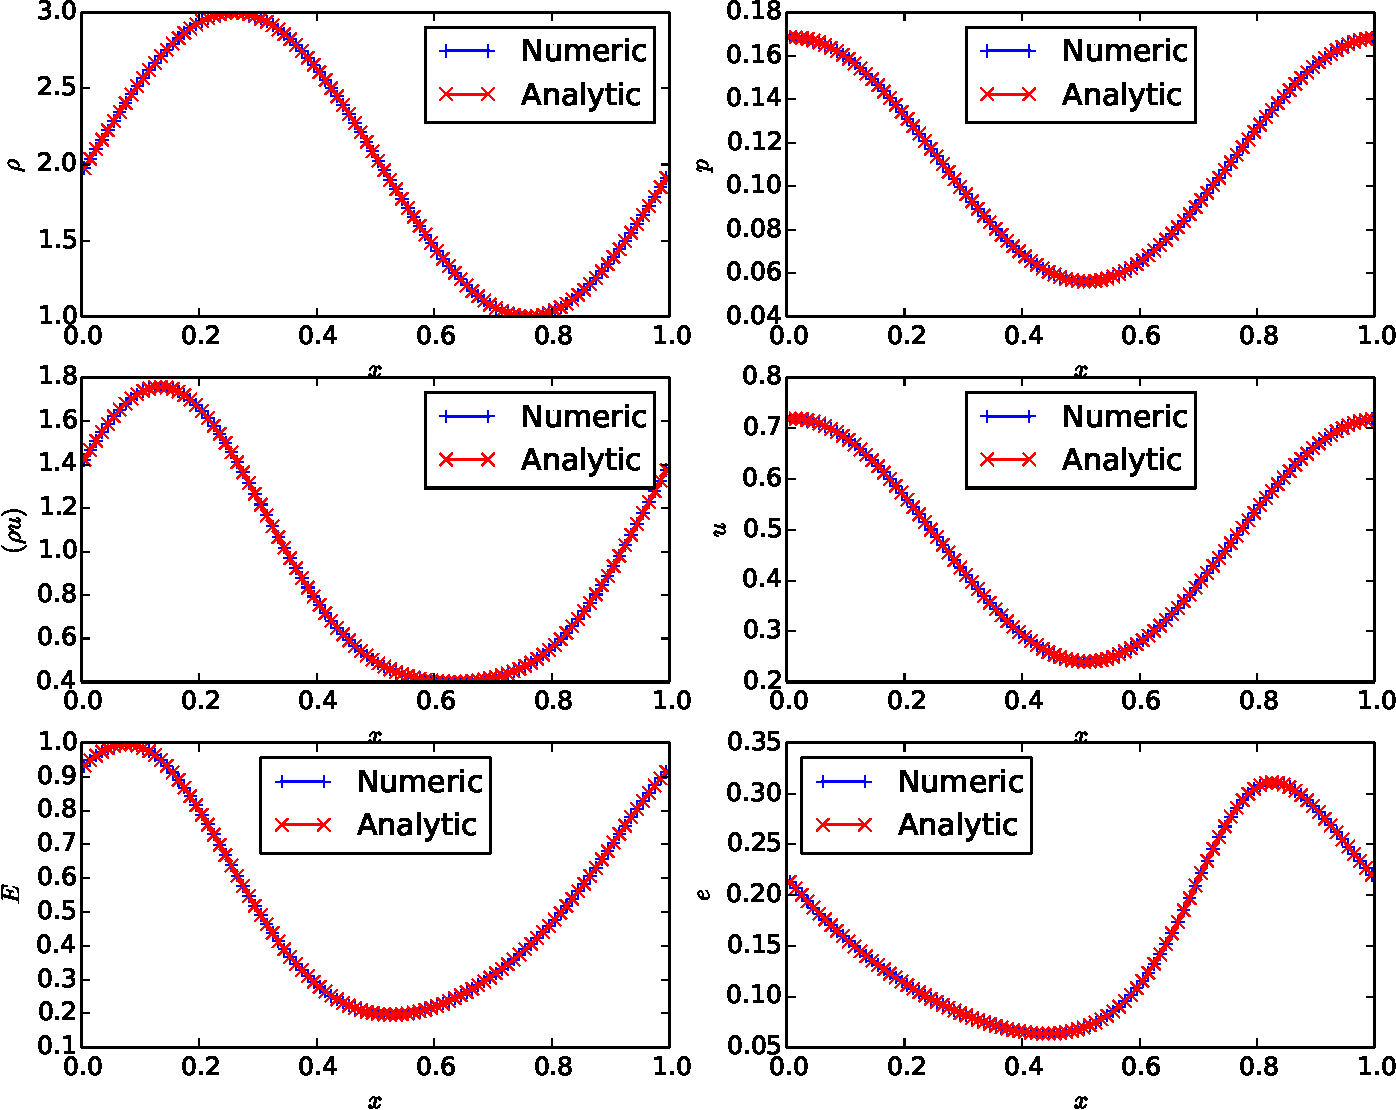
\includegraphics[width=\textwidth]{figures/MMS_diffusion_limit_solution.pdf}
   \caption{Hydrodynamic solution for the equilibrium diffusion limit MMS problem}
   \label{fig:MMS_diffusion_limit_solution}
\end{figure}

\begin{figure}[ht]
   \centering
   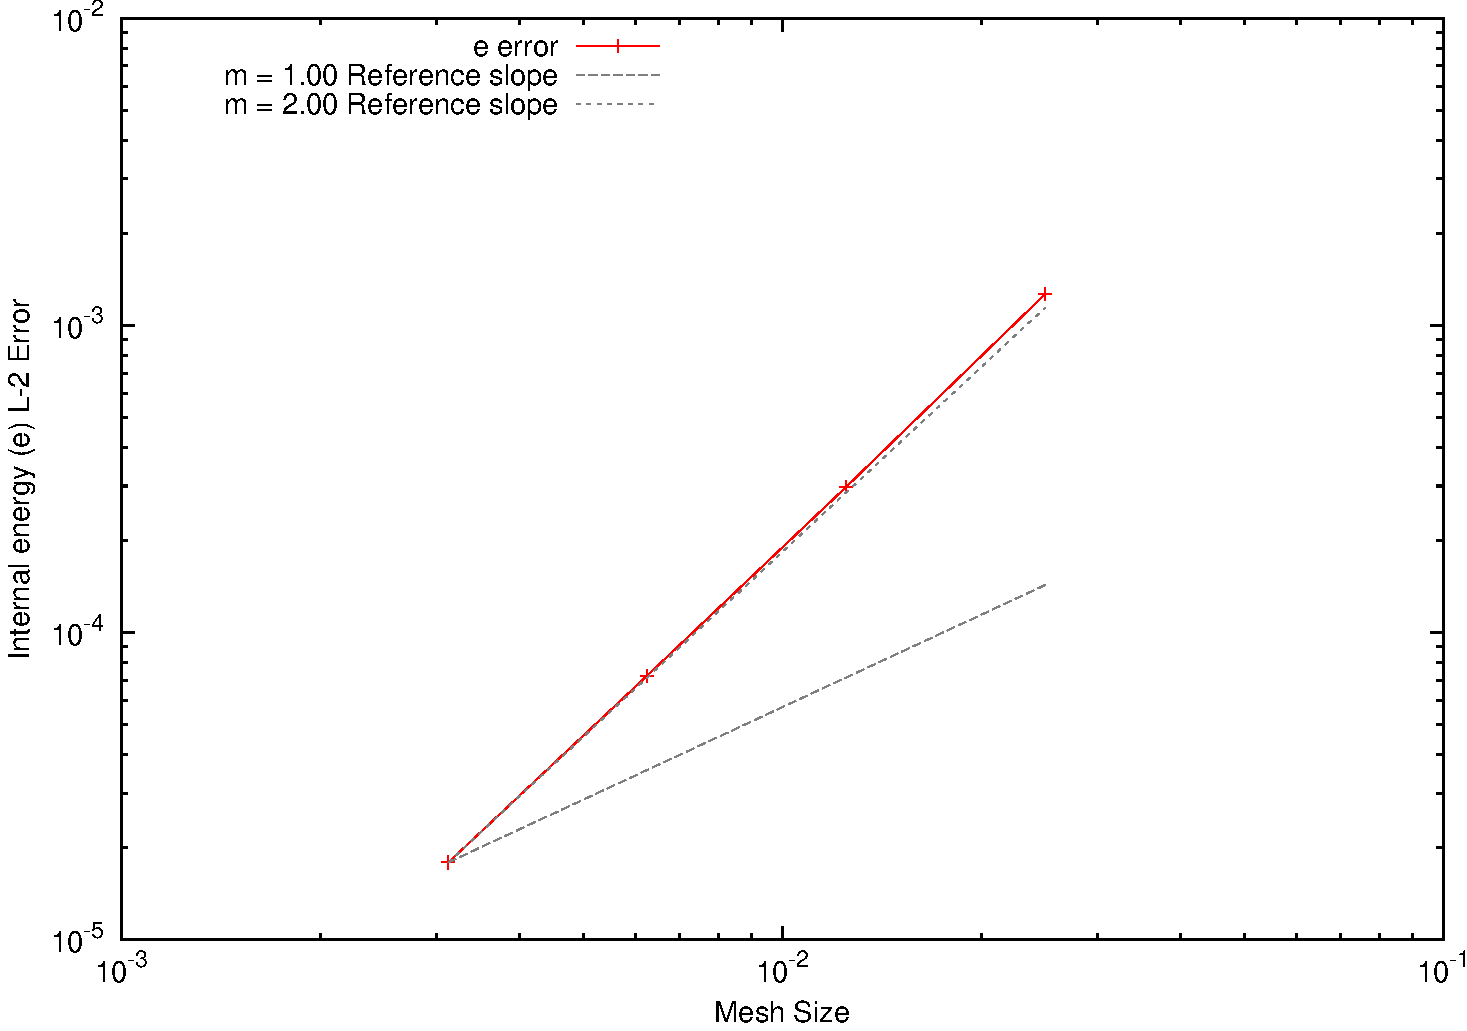
\includegraphics[width=\textwidth]{figures/MMS_diffusion_limit_convergence.pdf}
   \caption{Convergence of internal energy for the equilibrium diffusion limit MMS problem}
   \label{fig:MMS_diffusion_limit_convergence}
\end{figure}

The second MMS problem corresponds to the streaming limit, in which the radiation
and hydrodynamics are weakly coupled due to the high radiation energy propagation
speed relative to the fluid speed. For this problem, the following MMS solutions
are chosen:



\subsection{Streaming Limit}

Next, we consider the manufactured solution for the streaming limit.  In this limit, radiation streaming dominates a relatively small radiation absorption/re-emission term.  Here, we keep the re-emission term small by making the opacity relatively small so that the radiation is nearly transparent to the fluid.  Therefore, in contrast to the equilibrium diffusion limit which represents very tight coupling between the radiation and hydrodynamic components, this limit represents very weak coupling between the two.  Also, because the radiation streams much faster than the fluid, this results in a solution in which the unknowns evolve at significantly different time scales.  The functional form of the exact streaming solution is given by:

Here, was can see that the wave speed of the radiation energy density is faster than that of the hydrodynamic unknowns by a factor of $\mathbb{C}$.  This solution is also defined to mimic an isothermal flow regime, in which the radiation varies rapidly enough that changes in the fluid temperature are suppressed. In this case, the exact solution for the fluid temperature is a constant given by:

\section{Results for Radiation-Hydrodynamic Shocks}
\label{sec:ShockSolutions}

Reproducing radiative shocks accurately, particularly in the optically thick regime, represents a challenging problem in the simulation of radiation hydrodynamics.  However, because many problems of interest include radiative shocks, it is imperative that a numerical scheme be able to meet these challenges well.  The widely used Zel'dovich and Raizer \cite{zeldovich} and Mihalas and Mihalas \cite{mihalas} provide the classic descriptions of radiative shocks.  The structure of optically thick radiative shocks, which we consider here, has been described in more detail by Drake in \cite{Drake} and by Lowrie and Edwards in \cite{lowrie3}.  In the remainder of this section, we demonstrate the capability of our rad-hydro algorithm to compute accurate radiative shock solutions by reproducing the semi-analytic shocks detailed in \cite{lowrie3} and comparing our results with those of a first-order scheme.

Here, we describe our procedure to generate the shocks and compare our computational results with the semi-analytic solutions.  We begin by computing the far-downstream fluid state associated with a prescribed set of far-upstream conditions.  As we previously mentioned, these far-upstream conditions, and subsequently, the radiative shock itself, are specified by the shock Mach number $M$, the parameters $\mathbb{P}$ and $\sigma_a$, and the radiative diffusivity $\kappa$, which is given by:

\be
\lequ{kappa_def}
\kappa = \frac{\hat{c}}{3\hat{\sigma_t}\hat{a_0}\hat{L}} \pep
\ee

The equations that describe the overall jump from the upstream to the downstream states are a modified version of the Rankine-Hugoniot conditions derived by equating the flux terms from the fluid conservation equations in the rad-hydro model.  These modified Rakine-Hugoniot conditions are given-by:

\begin{subequations}
\lequ{radhydro_jump}
\be
\left(\rho v\right)_0 = \left(\rho v\right)_1 \pec
\ee
\be 
\left(\rho v^2+p^*\right)_0 = \left(\rho v^2+p^*\right)_1 \pec
\ee
\be 
\left[\left(\rho E^*+p^*\right)v\right]_0 = \left[\left(\rho E^*+p^*\right)v\right]_1 \pec
\ee
\end{subequations}

\noindent where

\begin{subequations}
\lequ{radhydro_jump_defns}
\be
p^* = p+\third \mathbb{P}T^4 \pec
\ee
\be
e^* = e + \frac{1}{\rho} \mathbb{P}T^4 \pec
\ee
\be
E^* = e^* + \half v^2 \pep
\ee
\end{subequations}

In \cite{lowrie4}, Lowrie and Rauenzahn show that these equations may be manipulated algebraically to solve for $\rho_1$:

\be
\lequ{jump_rho}
\rho_1(T_1) = \frac{f_1(T_1)+\sqrt{f_1^2(T_1)+f_2(T_1)}}{6(\gamma-1)T_1} \pec
\ee

\noindent where

\begin{subequations}
\lequ{jump_rho_defs}
\be
f_1(T_1) = 3(\gamma+1)(T_1-1)-\mathbb{P}\gamma(\gamma-1)(7+T_1^4) \pec
\ee
\be
f_2(T_1) = 12(\gamma-1)^2 T_1 \left[3+\gamma\mathbb{P}\left(1+7T_1^4\right)\right] \pep
\ee
\end{subequations}

Furthermore, eliminating $v_1$ from the mass equation, substituting the result into the momentum equation, and rearranging terms, we have an equation for $T_1$:  

\be
\lequ{jump_T}
3\rho_1(\rho_1 T_1 - 1)+\gamma\mathbb{P}\rho_1 \left(T_1^4-1\right) = 3\gamma(\rho_1-1)M_0^2 \pep
\ee

Substituting \equ{jump_rho} into \equ{jump_T}, this results in a ninth-order polynomial, which may be solved numerically for $T_1$.  We initialize this solution procedure using an estimate for $T_1$ based on $\mathbb{P}$.  For ``small'' values of $\mathbb{P}$, we initialize using:

\be
\lequ{T1_smallP}
T_1^{est} = \frac{\left(1-\gamma+2\gamma M^2\right)\left(2+(\gamma-1)M^2\right)^2}{(\gamma+1)^2 M^2} \pep
\ee

For ``large'' values of $\mathbb{P}$, we estimate $T_1$ as:

\be
\lequ{T1_largeP}
T_1^{est} = \sqrt[4]{\frac{8\left(\frac{M^2}{(4/9)\mathbb{P}}-1\right)}{7}} \pep
\ee

In solving for $T_1$, we note that the numerical solver does not always converge to the same final value for $T_1$ for both initial estimates.  However, for the shocks considered here, in the case when the initial estimates lead to differing values of $T_1$, the final solution for one estimate is always non-physical. So in these cases, it is obvious which converged $T_1$ value is correct. 

Because our radiation-hydrodynamics method is developed in dimensional form, we must also define the characteristic values $\hat{\rho_0}$ and $\hat{T_0}$.  The remaining dimensionalized values are computed from the non-dimensional parameters as follows:

\begin{subequations}
\label{shock_dim_defs}
\be
\hat{\rho_1} = \rho_1 \hat{\rho_0} \pec
\ee
\be
\hat{T_1} = T_1 \hat{T_0} \pec
\ee
\be
\hat{a_0} = \sqrt{\frac{\hat{\alpha_r} \hat{T_0}^4}{\hat{\rho_0} \mathbb{P}}} \pec
\ee
\be
\hat{v_0} = M \hat{a_0} \pec
\ee
\be
\hat{v_1} = v_1 \hat{a_0} \pec
\ee
\be
C_v = \frac{\hat{a_0}^2}{\hat{T_0}\gamma\left(\gamma-1\right)} \pec
\ee
\be
\hat{\sigma_t} = \frac{c}{3\kappa\hat{a_0}} \pec
\ee
\be
\hat{\sigma_a} = \sigma_a \frac{\hat{a_0}}{c} \pep
\ee
\end{subequations}

We initialize each radiative shock calculation by setting the left half of the spatial domain equal to the far-upstream condition and the right half equal to the downstream condition.  At the boundary, we compute the fluxes using our standard Riemann solver, setting the hydrodynamic unknowns in a ghost cell just to the other side of the boundary equal to the far-stream conditions.  This adds stability to the evolution of the shock by reinforcing the steady-state solution while allowing \URL{propagating} waves to exit the domain.  \fig{hydro_boundary_illustration} illustrates this concept for the right boundary.  Here, we set the left unknown in an exterior ghost cell equal to the far-downstream conditions, $U_{downstream}$, and compute the boundary advection flux, $F_{N+1/2}$, using our Riemann solver.

\begin{figure}[ht!]
%\begin{spacing}{1.0}
\centering
%\includegraphics[scale=0.70]{./figures/Hydro_Boundary_Illustration.png}
\caption{\bf Illustration of the advection boundary conditions for the radiative shock calculations.} 
\lfig{hydro_boundary_illustration}
%\end{spacing}
\end{figure}

Because sharp slopes in LDFEMs can cause negativities in edge values, we monitor for negativities in the fluid temperature.  If a negative temperature is detected, we set all the slopes in that cell to zero so that the edge values are equal to the cell-averages.  This preserves energy conservation while eliminating non-physical temperatures at cell-edges.  

%\subsubsection{Time Step Control}
%\label{time_step_control_rh}
 
To compute the time steps during the calculation, we use an adaptive time step control scheme based on a user-specified ``target temperature change'', $\Delta T_{targ}$.  Again, for a given time step, the maximum relative change is computed using:
\be
\Delta T=2\max_i\frac{\abs{T_i^{n+1}-T_i^n}}{T_i^{n+1}+T_i^n} \pep
\lequ{max_delT_eqn_rh}
\ee

However, because we use an IMEX scheme to solve our rad-hydro system, we must also limit the time step according to the Courant limit associated with the hydrodynamic advection terms.  We compute this limit by determining the maximum signal velocity associated with the system and define the maximum hydrodynamic time step to be:

\be
\lequ{courant_limit}
\Delta t_H = CFL\Delta x S_{max} \pec
\ee

\noindent where $S_{max}$ is the maximum signal velocity, and $CFL$ is the user-defined Courant condition number such that $0\le C \le 1$.  We use the following estimate for $S_{max}$ outlined in \cite{toro}:

\be
\lequ{S_max}
S_{max} = \max_{i\in \bracket{1,N}}\bracet{\abs{u_i-a_i},\abs{u_i+a_i}} \pec
\ee

\noindent where $N$ is the number of cells, $u_i$ is the velocity in cell i, and $a_i$ is the speed of sound in cell i.  We then compute the time step as follows:

\be
\Delta t^{n+1}=\min\fn{\frac{\Delta T_{targ}}{\Delta T}\Delta t^{n}, \xi \Delta t^n, \Delta t_H, t-t_{fin}} \pep
\lequ{time_control_rh}
\ee

The second term ensures that the time step doesn't grow too rapidly by imposing a maximum allowed time step change, $\xi$, and the fourth term forces the final time step to end the calculation at $t_{fin}$.  In order to ensure that the temperature doesn't vary too much, $\Delta T$ is also compared with a maximum allowed temperature change, $\Delta T_{max}$.  If $\Delta T > \Delta T_{max}$, then the time step $\Delta t^{n+1/2}$ is reduced by a factor of 1/3, and the calculation is repeated from $t_n$.  In our calculations, we set $CFL = 0.3$, $\Delta T_{targ} = 1.01$, $\Delta T_{max} = 1.012$, and $\xi = 1.5$.

\subsection{Radiative Shock Solutions}
\label{sec:radshocksols}

We test our algorithm over a range of the radiative shocks presented in \cite{lowrie3}, which incorporate a variety of structural features.  For each of these shocks, we set $\mathbb{P} = 1e-4$, $\gamma = 5/3$, $\kappa = 1$, and $\sigma_a = 1e6$, and the fluid properties are given in \ta{matl_prop}. 

%We test our algorithm using two of the radiative shocks presented in \cite{lowrie3}.  The Mach 2 shock solution shows the full complexity in the shock structure, and the Mach 50 shock is the most computationally challenging to solve.  For each of these shocks, we set $\mathbb{P} = 1e-4$, $\gamma = 5/3$, $\kappa = 1$, and $\sigma_a = 1e6$, and the fluid properties are given in \ta{matl_prop}. 

\begin{table}
\centering
\caption{\bf fluid properties for radiative shock calculations.}
\lta{matl_prop}
\begin{tabular}{|c|c|}
\hline
$\hat{\sigma_a}$ & 3.9071164263502112e+002 \\
$\hat{\sigma_t}$ & 8.5314410158161809e+002 \\
$\hat{C_v}$ & 1.2348000000000001e-001 \\
\hline
\end{tabular}
\end{table}

%\rev{We begin by reproducing the Mach 1.05 shock, which has no hydrodynamic shock and no ISP.  \ta{mach105_initconds} details the initial fluid properties, and the final time of the calculation is 2.5 shakes.  Computationally, this is the easiest of the shocks to compute, since the small difference between the upstream and downstream values lends to a smooth transition period from the initial conditions to the steady-state solution.  As we see in \fig{mach105_rho} for the density and \fig{mach105_T} for the fluid and radiation temperatures, our results match the semi-analytic solutions well.  Here, we can see that the fluid properties are continuous, due to the lack of a hydrodynamic shock, and the maximum fluid temperature never exceeds the far-downstream temperature, since there is no ISP.} 

%\begin{table}
%\centering
%\caption{\bf Mach 1.05 initial conditions.}
%\lta{mach105_initconds}
%\begin{tabular}{|c|c|c|}
%\hline
% & Pre-shock & Post-shock \\
%\hline
%$\hat{\rho}$ & 1.0000000000000000e+00 & 1.0749588725963066e+000 \\
%$\hat{u}$ & 1.2298902390050911e-001 & 1.1441277153558302e-001 \\
%$\hat{T}$ & 1.0000000000000001e-001 & 1.0494545175154467e-001 \\
%$\hat{\rho} \hat{u}$ & 1.2298902390050911e-001 & 1.2298902390050913e-001 \\
%$\hat{E}$ & 1.9911150000000002e-002 & 2.0965788801187071e-002 \\
%$\hat{E_r}$ & 1.3720000000000002e-006 & 1.6642117992569650e-006 \\
%$4/3 \hat{E} \hat{u}$ & 2.2498792105533135e-007 & 2.5387611250027822e-007 \\
%\hline
%\end{tabular}
%\end{table}

%\begin{figure}[ht!]
%%\begin{spacing}{1.0}
%\centering
%\includegraphics[scale=0.60]{./figures/Mach_1p05_rho.png}
%\caption{\bf Mach 1.05 radiative shock density.} 
%\lfig{mach105_rho}
%%\end{spacing}
%\end{figure}

%\begin{figure}[ht!]
%%\begin{spacing}{1.0}
%\centering
%\includegraphics[scale=0.60]{./figures/Mach_1p05_T.png}
%\caption{\bf Mach 1.05 radiative shock fluid and radiation temperatures.} 
%\lfig{mach105_T}
%%\end{spacing}
%\end{figure}
%%

%\FloatBarrier
First, we compute the Mach 1.2 shock, which has a hydrodynamic shock but no ISP.  \ta{mach12_initconds} shows the initial conditions; the final time of the calculation is 0.5 shakes.  \figs{mach12_rho} and \rfig{mach12_T} compare our results with the semi-analytic solutions for the density and fluid and radiation temperatures, respectively, and again, we see good agreement between the two.  In this solution, we see a discontinuity in both the density and fluid temperature due to the hydrodynamic shock, and the maximum temperature is bounded by the far-downstream temperature, since there is no ISP to drive it further.


A Mach 2 radiative shock problem was taken from \cite{edwardsthesis}.
The material properties are uniform and are given in Table
\ref{tab:mach2_shock_material}. Initial conditions in the pre-shock
and post-shock regions are given in Table \ref{tab:mach2_shock_IC}.
Figure \ref{fig:mach2_shock_T} shows the numerical solution computed
with 300 cells and a CFL of 0.6, using the van Leer slope limiter;
the comparison to the reference solution shows excellent agreement.

\begin{table}[ht]
  \centering
  \caption{Material property values for the Mach 2 radiative shock problem}
  \label{tab:mach2_shock_material}
  \begin{tabular}{l l}\hline
    \emph{Parameter} & \emph{Value}\\\hline
    $\sigma_a$ & 390.71164263502112\\
    $\sigma_t$ & 853.14410158161809\\
    $c_v$      & 0.12348\\\hline
  \end{tabular}
\end{table}

\begin{table}[ht]
  \centering
  \caption{Initial condition values for the Mach 2 radiative shock problem}
  \label{tab:mach2_shock_IC}
  \begin{tabular}{l l l}\hline
    \emph{Parameter} & \emph{Pre-shock Value} & \emph{Post-shock Value}\\\hline
    $\rho$           & 1                      & 2.2860748989303659\\
    $u$              & 0.23426480742954117    & 0.10247468599526272\\
    $E$              & 3.9788000000000004e-2  & 7.0649692950433357e-2\\
    $\E$             & 1.3720000000000002e-6  & 2.5560936967521927e-5\\
    $\F$             & 0                      & 0\\\hline
  \end{tabular}
\end{table}

\begin{figure}[ht]
   \centering
   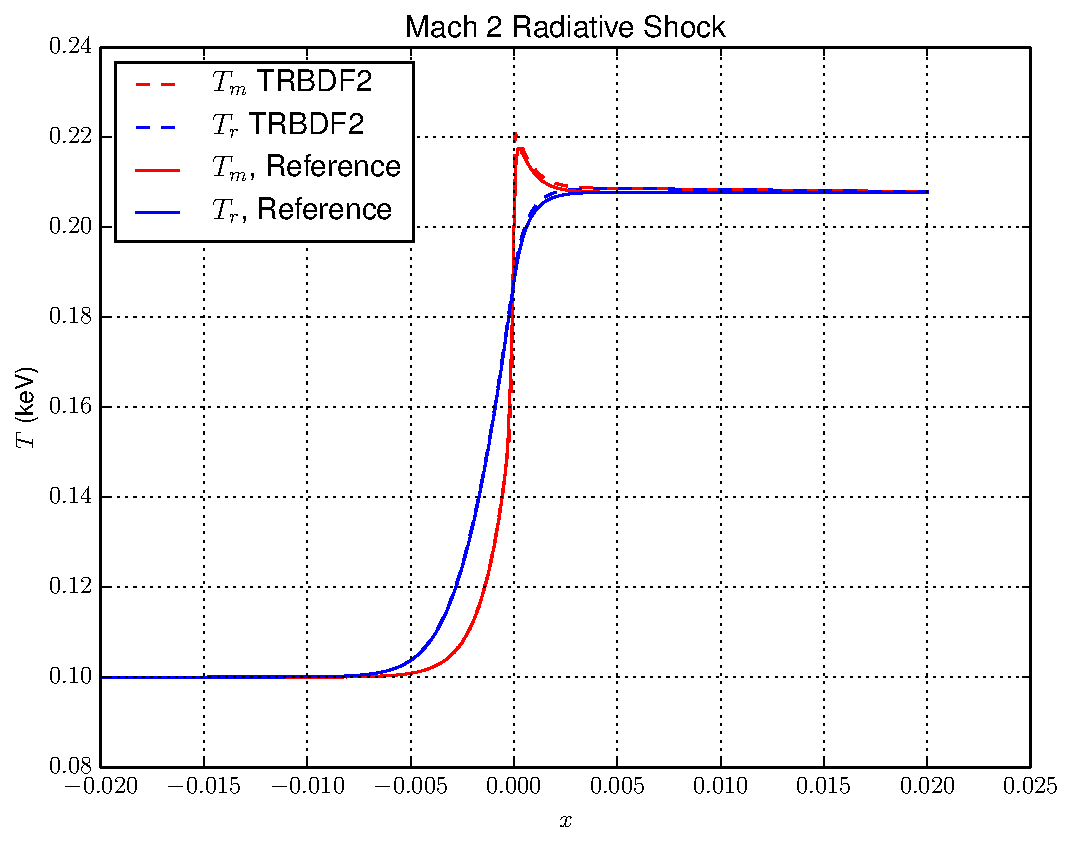
\includegraphics[width=\textwidth]{figures/mach2_shock_T.pdf}
   \caption{Comparison of Mach 2 radiative shock solution to reference solution}
   \label{fig:mach2_shock_T}
\end{figure}



The most structurally complex shock that we compute is the Mach 2 shock, which has both a hydrodynamic shock and an ISP.  The initial conditions are given by \ta{mach2_initconds}, and the final time of the calculation is 1 shake.  \figs{mach2_rho} and \rfig{mach2_T} show our results compared with the semi-analytic solutions.  In each of these figures, we can see the effects of the hydrodynamic shock, causing a discontinuity in both the fluid density and temperature.  We can also see the Zel'dovich spike, caused by the ISP embedded within the hydrodynamic shock, driving up the fluid temperature at the shock front.  This spike leads to the relaxation region downstream as the fluid temperature and radiation temperature equilibrate. \fig{mach2_spike} shows the Zel'dovich spike and relaxation region in more detail. Here, we can see that our results still show very good agreement with the semi-analytic solution.





\section{Conclusions and Future Work}


\bibliographystyle{model1-num-names}
\bibliography{References}


\clearpage

\appendix
\section{Details of the Radiation-Hydrodynamics Method}
Here we give a detailed description of our radiation-hydrodynamics method.
First, we define some notation; the following are quantities stored
throughout the calculation:
\begin{center}
\begin{tabular}{l|l}
   Radiation angular intensities & $\R^n \equiv \{\Psi^\pm\iL,\Psi^\pm\iR\} \quad\forall i$ \\
   Conservative hydrodynamics variables & $\H^n \equiv \{\rho_i^n, (\rho u)_i^n, E_i^n\} \quad\forall i$ \\
   MHM fluid internal energy slopes & $\delta e^n \equiv \{\delta e_i^n\} \quad\forall i$ \\
   MHM conservative variable slopes & $\bar{\Delta}^n \equiv \{\bar{\Delta}\rho_i^n, \bar{\Delta}(\rho u)_i^n,
     \bar{\Delta} E_i^n\} \quad\forall i$ \\
   Macroscopic cross sections & $\sigma^n \equiv \{\sigma_{s,i,L}^n, \sigma_{s,i,R}^n,
   \sigma_{a,i,L}^n, \sigma_{a,i,R}^n, \sigma_{t,i,L}^n, \sigma_{t,i,R}^n\}
   \quad\forall i$
\end{tabular}
\end{center}
Other quantities are computed when needed.
The solution for a time step $t^n\rightarrow t^{n+1}$ consists of four
nonlinear solves:
\begin{enumerate}
  \item Crank-Nicolson step from $t^n$ to $t^{n+\fourth}$
    (Cycle 1 Predictor)
  \item Crank-Nicolson step from $t^n$ to $t^{n+\half}$
    (Cycle 1 Corrector)
  \item Crank-Nicolson step from $t^{n+\half}$ to $t^{n+\frac{3}{4}}$
    (Cycle 2 Predictor)
  \item TR/BDF-2 step from $t^{n+\half}$ to $t^{n+1}$
    (Cycle 2 Corrector)
\end{enumerate}

\begin{enumerate}




% Cycle 1 predictor

\item \textbf{Perform Cycle 1 Predictor.} 
\begin{enumerate}
\item \textbf{Perform MUSCL-Hancock Predictor.} First, slopes $\Delta^n$ are
computed via Equations \eqref{eq:muscl_slopes} and \eqref{eq:muscl_differences},
optionally applying a slope limiter.
Then a linear-discontinuous representation of the solution is created via
Equation \eqref{eq:edge_hydro}, and the
the MUSCL-Hancock predictor is performed to obtain $\H^*$, the
homogeneous hydrodyamics solution at $t^{n+\fourth}$,
via Equation \eqref{eq:muscl_predictor}.

\item \textbf{Perform nonlinear iterations.} Iteration of the
$t^{n+\fourth}$ solution is required since the system of equations
is nonlinear. 
\begin{enumerate}
\item\label{item:vel_update}
\textbf{Update velocities.} The Crank-Nicolson discretization
of the velocity update equation, Equation \requ{hydromCNfull},
is solved to obtain new
velocities at cell centers, $\{u_i^{k+1}\}$. Evaluation of
the radiation quantities $\E$ and $\F$
at cell centers is achieved by averaging the left and right values.

\item \textbf{Update radiation.} The Crank-Nicolson discretization of the S-2
equations, Equations \requ{S2CNfullL} and \requ{S2CNfullR} are solved,
employing the linearization given in Section \ref{sec:linearization}.
Evaluation of the densities and velocities at the edges is achieved using using
the cell-centered values in conjunction with the slopes $\Delta^n$. Evaluation
of the material energy $E$ at edges is achieved using the internal energy
slopes $\delta e^n$ from a previous radiation solve.  The computation of this
slope is described in Section~\ref{sec:e_slopes}.

\item \textbf{Update internal energies.} The internal energies are
updated in accordance with the linearization procedure given is Section
\ref{sec:linearization}. The update equations produce edge values
$\{e^{k+1}\iL,e^{k+1}\iR\}$. These left and right values are added to the 
kinetic energy at edges to produce cell-averaged values for the total energy
$\{E^{k+1}_i\}$, which are used in the subsequent iteration.  The values
of $\delta e$ are stored for the next radiation solve.
Cross sections that are updated if they are functions of the hydrodynamic 
state of the fluid.

\item \textbf{Check convergence.} The new solutions $\R^{k+1}$ and
$\H^{k+1}$ are compared with the previous iteration solutions
$\R^k$ and $\H^k$ to determine if convergence has been achieved.
If the solutions have not converged, then the computation
returns to Step \ref{item:vel_update}.
\end{enumerate}
\end{enumerate}

% Cycle 1 corrector

\item \textbf{Perform Cycle 1 Corrector.} This step proceeds
just as the predictor step, except that the MUSCL-Hancock
corrector step given by Equation \eqref{eq:muscl_corrector} is used instead of the MUSCL-Hancock predictor
step, and the step goes from $t^n$ to $t^{n+\half}$ instead
of $t^n$ to $t^{n+\fourth}$. No new hydrodynamic slopes are computed;
evaluation of edge densities and velocities use
$\Delta^n$.  However, evaluation of edge internal energies
in the nonlinear iteration use $\delta e^{n+1/4}$ (CURRENTLY WE JUST USE $\delta
e^{n}$, NEED TO CHECK THIS). At the end
of the cycle, the new internal energy slopes $\delta e^{n+\half}$
are saved for the next cycle.

% Cycle 2 predictor

\item \textbf{Perform Cycle 2 Predictor.} This step proceeds
just as the Cycle 1 predictor step, except that the
step goes from $t^{n+\half}$ to $t^{n+\frac{3}{4}}$ instead
of $t^n$ to $t^{n+\fourth}$. As in Cycle 1, new slopes
are computed in the MUSCL-Hancock predictor step;
these slopes $\Delta^{n+\half}$ are then used for
evaluation of edge densities and velocities in the remainder
of the cycle. Evaluation of edge internal energies
and temperatures use the internal energies saved
from the end of Cycle 1, $\delta e^{n+\half}$.

% Cycle 2 corrector

\item \textbf{Perform Cycle 2 Corrector.} This step proceeds
as the Cycle 1 corrector step, except that the time step goes
from $t^{n+\half}$ to $t^{n+1}$, and the time discretization
of the equations is a form of TR/BDF-2
instead of Crank-Nicolson, so values at $t^n$
are used in the temporal discretization. Slopes
$\Delta^{n+\half}$ and $\delta e^{n+\frac{3}{4}}$ (CURRENTLY WE JUST USE $\delta
e^{n+\half}$, NEED TO CHECK THIS) are again
used to evaluate edge quantities. At the end
of the cycle, the new internal energy slopes $\delta e^{n+1}$
are saved for the next cycle.

% End

\item \textbf{Store values for next time step.}
At this point, the old solutions, hydrodynamics slopes,
internal energy slopes, and cross sections
are saved for the next time step.

\end{enumerate}

%===============================================================================
\section{The Discretized Equations}\lsec{full}
%===============================================================================
%===============================================================================
\subsection{MUSCL-Hancock Equations}
%===============================================================================

The homogeneous Euler equations may be expressed in conservative form as
\begin{equation}
  \dydt{\H} + \nabla\cdot\Flux(\H) = \mathbf{0} \pec
\end{equation}
where $\H$ is a vector of the conservative unknowns
and $\Flux(\H)$ is the flux associated with each:
\begin{equation}
  \H=\left[\begin{array}{c}\rho\\\rho u\\E\end{array}\right] \pec\qquad
  \Flux(\H)=\left[\begin{array}{c}\rho u\\
  \rho u^2 + p\\
  (E+p)u\end{array}\right] \pep
\end{equation}
The first half of a MUSCL-Hancock step $t^n\rightarrow t^n+\dt$
starts by constructing a linear representation of the solution
using slopes $\Delta_i^n$:
\begin{equation}\label{eq:muscl_slopes}
  \Delta_i^n = \half\Delta\H_{i-\half}^n + \half\Delta\H_{i+\half}^n \pec
\end{equation}
\begin{equation}\label{eq:muscl_differences}
  \Delta\H_{i-\half}^n = \H_i^n - \H_{i-1}^n \pec\quad
  \Delta\H_{i+\half}^n = \H_{i+1}^n - \H_i^n \pec
\end{equation}
These slopes are optionally limited via slope limiters $\xi_i$:
\begin{equation}
  \bar{\Delta}_i = \xi_i \Delta_i \pep
\end{equation}
We have chosen to use the double-minmod slope limiter~\cite{ref???}.
If no slope limiter is used, then $\xi_i=1$. The linear representation
of the solution is built as
\begin{equation}\label{eq:edge_hydro}
  \H\iL^n = \H_i^n - \frac{\bar{\Delta}_i^n}{2} \pec
  \quad
  \H\iR^n = \H_i^n + \frac{\bar{\Delta}_i^n}{2} \pec
\end{equation}
This representation is then evolved by half a time step:
\hydroPredictor{n}{n+\half}{\half}{\label{eq:muscl_predictor}}
The second half of a MUSCL-Hancock step employs a Riemann solver
to compute the fluxes at time $n+\half$:
\hydroCorrector{n}{n+\half}{n+1}{}{\label{eq:muscl_corrector}}

%===============================================================================
%\subsubsection{Slope Limiters}\label{sec:slope_limiters}
%===============================================================================
%See Jarrod's memo.

%-------------------------------------------------------------------------------
\subsection{Fluid Momentum Source Update Equation}
%-------------------------------------------------------------------------------
The Crank-Nicolson discretization of the velocity update equation is the
following:
\momentumUpdateCN{n}{}{_i}{\lequ{hydromCNfull}}
The BDF2 discretization of the velocity update equation is the
following:
\momentumUpdateBDFTwo{n-1}{n}{}{_i}{\lequ{hydromBDF2full}}
The momentum source terms in these equations are computed by taking the linear
average of the momentum source expressions evaluated at the edges, e.g., 
\begin{multline}
   \left[\frac{\sigma_t}{c}\left(\F - \frac{4}{3}\E u\right)\right]_i =
   \half\left[\frac{\sigma_{t,i,L}}{c}\left(\F\iL - \frac{4}{3}\E\iL u\iL\right)\right]\\
   + \half\left[\frac{\sigma_{t,i,R}}{c}\left(\F\iR - \frac{4}{3}\E\iR u\iR\right)\right]
   \pep
\end{multline}

%-------------------------------------------------------------------------------
\subsection{Fluid Energy Source Update Equation}
%-------------------------------------------------------------------------------
The energy source update equations are evaluated at the edges and thus hydrodynamic
quantities need to be evaluated at the edges. The stored solution values
consist of the cell average unknowns for the conservative variables $[\rho,\rho u,E]$
and their slopes $\Delta$, which come from the predictor step of MUSCL-Hancock,
as given by Equation \eqref{eq:muscl_slopes}. Evaluation of edge densities is achieved
by applying the slopes as given by Equation \eqref{eq:edge_hydro}:
\begin{equation}
   \rho\iL^k = \rho_i^k - \frac{\Delta\rho_i^n}{2} \pep
\end{equation}
Note that the slopes $\Delta$ are only updated in the MUSCL-Hancock predictor
step. Thus, quantities at $t^{n+1}$ also use the $\Delta^n$ slopes. For the
BDF2 discretization, where evaluation of quantities at $t^{n-1}$ is required,
the old slopes $\Delta^{n-1}$ are used. Evaluation of edge velocities is
achieved by evaluating the edge conservative variables $\rho$ and $\rho u$
and then computing velocity from these, e.g.,
\begin{equation}
   u\iL^k = \frac{(\rho u)\iL^k}{\rho\iL^k}
          = \frac{(\rho u)_i^k - \frac{\Delta(\rho u)_i^n}{2}}
                 {\rho_i^k - \frac{\Delta\rho_i^n}{2}} \pep
\end{equation}
As explained in Section~\ref{sec:e_slopes}, internal energy unknowns, and thus material
temperature, use slopes that are independent of the MUSCL-Hancock slopes.
These internal energy slopes are denoted by $\delta e$. Evaluation
of edge internal energies is thus performed as follows:
\begin{equation}
   e\iL^k = e_i^k - \frac{\delta e_i^n}{2} \pep
\end{equation}
Edge temperatures are computed from the edge internal energies:
\begin{equation}
   T\iL^k = \frac{e\iL^k}{c_v} \pep
\end{equation}
Again, quantities at $t^{n+1}$ still use old slopes $\delta e^n$. These
slopes are updated at the end of each full MUSCL-Hancock step, i.e.,
when the nonlinear iteration for the corrector step converges, the
slopes $\delta e_i^{n+1}$ are computed from the converged edge internal energies:
\begin{equation}
   \delta e_i^{n+1} = e\iR^{k+1} - e\iL^{k+1} \pep
\end{equation}
The Crank-Nicolson discretization of the energy update equation is
\energyUpdateCN{n}{}{\iL}{\lequ{hydroECNfull}}
The right edge equations are identical in form, obtained by replacing ``$L$'' with
``$R$'' in the left edge equations.
The BDF2 discretization of the energy update equation is
\energyUpdateBDFTwo{n-1}{n}{}{\iL}{\lequ{hydroEBDF2full}}
The energy update to the 
Note that these energy update equations are not in the form in which they
are actually solved in practice; the implicit term $\sigma_a^k a c (T^{k+1})^4$
must be linearized. This procedure is detailed in Section \ref{sec:linearization}.
The final form of the energy update equation is a direct update to the
edge internal energies $\{e\iL^{k+1},e\iR^{k+1}\}$.

\subsection{Using Radiation Internal Energy Slopes}
\label{sec:e_slopes}

As discussed in the introduction, the radiation solver and hydro solver use different
internal energy slopes as an approach to preserve the equilibrium diffusion limit.   The
implementation of separate slopes is a proof of concept for higher dimensions.
To mitigate confusion, in this section we will denote the hydro-state internal energy variables as $e$ and
the internal energy variables coming from the non-linear radiation solves as $e^r$. Care must be taken to
ensure that total energy is conserved.  The modified slopes are only applied to the implicit terms in each
nonlinear solve.

During the MHM solve, we
use the standard slope reconstruction formulas to advect variables to
state $U^*$ (or $U^{**}$), including total energy $E$.  Then, in the non-linear iteration loop for the radiation
and internal energy densities we use a modified slope for $E^*$, denoted $\Delta E^{r*}$, that will preserve the diffusion
limit.  This $\Delta E^{r*}$ is based on the edge values of $e^r$ of \emph{the last iteration of the previous
nonlinear radiation solve}.  For example, if we are solving the cycle 1 corrector from state $e^*$ to
$e^{n+1/2}$, we use the edge values of $e^r$ from the last iteration of the solve for
$e^{r,n+1/4}$ to construct the slopes for $\Delta E^{r,*}$. The value of $\Delta
E^{r,*}$ does not change over the duration of the nonlinear solve.

For the nonlinear solve we need the to use $\delta e^r$ to construct
$\Delta E^{*r}$ in the next solve (and thus the values $E^*_{R/L} = E^*_i \pm \frac{1}{2}\Delta E^{r*}$
needed for the LD radiation solve).  We approximate this slope based on the hydro values
for $E^*$ as:
\begin{equation}
    \Delta E^{r*} = E^{r*}_R - E^{r*}_L
\end{equation}
where 
\begin{equation}\label{estarr}
    E^{r*}_R = \rho^*_R\left((u_R^*)^2 + e^*_i +
    \delta e^{r,n+1/4}\right),
\end{equation}
\begin{equation}\label{estarl}
    E^{r*}_L = \rho^*_R\left((u_L^*)^2 + e^*_i -
    \delta e^{r,n+1/4}\right),
\end{equation}
and subscript $i$ denotes cell average quantities.  The edge values of $\rho$ and
$u$ are evaluated using the MHM slopes as usual.
 Once we have completed
the nonlinear solve for $e^{r,n+1/2}_{L/R}$, we must compute the change made to the
cell-averaged total energy for the next MHM solve, such that total energy is conserved. The formula for the new total energy is
\begin{equation}\label{ei}
    E^{n+1/2}_i = \frac{1}{2}\left[\rho_L\left(\frac{1}{2}u_L^2 + e_L^r\right)
    +\rho_R\left(\frac{1}{2}u_R^2 + e_R^r\right)\right]^{n+1/2}
\end{equation}
where all variables are at time $t^{n+1/2}$. The internal energy slopes are computed
and stored for the next nonlinear solve.  For the first solve, the internal energy
slopes are assumed zero.


%-------------------------------------------------------------------------------
\subsection{\texorpdfstring{S$_2$}{S-2} Equations}
%-------------------------------------------------------------------------------

A lumped linear discontinuous (LLD) spatial discretization is employed
for the S$_2$ equations, so the angular flux
unknowns are the left and right values $\Psi_{i,L}^\pm$ and
$\Psi_{i,R}^\pm$ for each cell $i$. The spatially
discretized equations result from integrating each half cell
$(x_i-\frac{h_i}{2},x_i)$ and $(x_i,x_i+\frac{h_i}{2})$,
where $x_i$ is the cell center, $h_i$ is the cell width,
and the cell average and edge fluxes are defined as
\begin{equation}
  \Psi_i^\pm=\half\fn{\Psi_{i,L}^\pm + \Psi_{i,R}^\pm} \pec
\end{equation}
\begin{equation}
  \Psi_{i+\half}^+=\Psi_{i,R}^+ \pec\qquad \Psi_{i+\half}^-=\Psi_{i+1,L}^- \pep
\end{equation}

%===============================================================================
\subsubsection{Steady-State}\lsec{S2ssdisc}
%===============================================================================
Using an LLD discretization, the steady-state S$_2$ equations, obtained by
dropping the $\dydt{\Psi^\pm}$ term in Equation \requ{S2Q}, become
\begin{equation}\lequ{S2ssL}
  \frac{2\mu^\pm}{h_i}\fn{\Psi^{\pm,k+1}_i - \Psi^{\pm,k+1}_{i-\half}}
  +\sigma_{t,i,L}^k\Psi\iL^{\pm,k+1}
  -\frac{\sigma_{s,i,L}^k}{2}\phi\iL^{k+1}
  =\Q_{i,L}^{\pm,k} \pec
\end{equation}
\begin{equation}\lequ{S2ssR}
  \frac{2\mu^\pm}{h_i}\fn{\Psi^{\pm,k+1}_{i+\half} - \Psi^{\pm,k+1}_i}
  +\sigma_{t,i,R}^k\Psi\iR^{\pm,k+1}
  -\frac{\sigma_{s,i,R}^k}{2}\phi\iR^{k+1}
  =\Q_{i,R}^{\pm,k} \pep
\end{equation}



\subsubsection{Crank-Nicolson}\lsec{S2fullCN}
%-------------------------------------------------------------------------------
\begin{equation}\lequ{S2CNfullL}\begin{split}
  \frac{1}{c}\frac{\Psi\iL^{\pm,k+1}-\Psi\iL^{\pm,n}}{\dt} = &
  -\half\frac{2\mu^\pm}{h_i}\fn{\Psi^{\pm,n}_i - \Psi^{\pm,n}_{i-\half}}
  -\half\frac{2\mu^\pm}{h_i}\fn{\Psi^{\pm,k+1}_i - \Psi^{\pm,k+1}_{i-\half}}\\
  &-\half\sigma_{t,i,L}^n\Psi\iL^{\pm,n}
   -\half\sigma_{t,i,L}^k\Psi\iL^{\pm,k+1}\\
  &+\half\frac{\sigma_{s,i,L}^n}{2}\phi\iL^n
   +\half\frac{\sigma_{s,i,L}^k}{2}\phi\iL^{k+1}\\
  &+\half\Q_{i,L}^{\pm,n}
   +\half\Q_{i,L}^{\pm,k} \pep
\end{split}\end{equation}

\begin{equation}\lequ{S2CNfullR}\begin{split}
  \frac{1}{c}\frac{\Psi\iR^{\pm,k+1}-\Psi\iR^{\pm,n}}{\dt} = &
  -\half\frac{2\mu^\pm}{h_i}\fn{\Psi^{\pm,n}_{i+\half} - \Psi^{\pm,n}_i}
  -\half\frac{2\mu^\pm}{h_i}\fn{\Psi^{\pm,k+1}_{i+\half} - \Psi^{\pm,k+1}_i}\\
  &-\half\sigma_{t,i,R}^n\Psi\iR^{\pm,n}
   -\half\sigma_{t,i,R}^k\Psi\iR^{\pm,k+1}\\
  &+\half\frac{\sigma_{s,i,R}^n}{2}\phi\iR^n
   +\half\frac{\sigma_{s,i,R}^k}{2}\phi\iR^{k+1}\\
  &+\half\Q_{i,R}^{\pm,n}
   +\half\Q_{i,R}^{\pm,k} \pep
\end{split}\end{equation}


\subsubsection{TR/BDF-2}\lsec{S2fullTRBDF2}
%-------------------------------------------------------------------------------
\begin{equation}\lequ{S2BDF2fullL}\begin{split}
  \frac{1}{c}\frac{\Psi\iL^{\pm,k+1}-\Psi\iL^{\pm,n}}{\dt} = &
   -\sixth     \frac{2\mu^\pm}{h_i}\fn{\Psi^{\pm,n-1}_i - \Psi^{\pm,n-1}_{i-\half}}
   -\sixth     \frac{2\mu^\pm}{h_i}\fn{\Psi^{\pm,n}_i   - \Psi^{\pm,n}_{i-\half}}\\
  &-\frac{2}{3}\frac{2\mu^\pm}{h_i}\fn{\Psi^{\pm,k+1}_i - \Psi^{\pm,k+1}_{i-\half}}\\
  &-\sixth\sigma_{t,i,L}^{n-1}\Psi\iL^{\pm,n-1}
   -\sixth\sigma_{t,i,L}^{n}  \Psi\iL^{\pm,n}
   -\frac{2}{3}\sigma_{t,i,L}^k\Psi\iL^{\pm,k+1}\\
  &+\sixth\frac{\sigma_{s,i,L}^{n-1}}{2}\phi\iL^{n-1}
   +\sixth\frac{\sigma_{s,i,L}^{n}}{2}  \phi\iL^{n}
   +\frac{2}{3}\frac{\sigma_{s,i,L}^k}{2}\phi\iL^{k+1}\\
  &+\sixth\Q_{i,L}^{\pm,n-1}
   +\sixth\Q_{i,L}^{\pm,n}
   +\frac{2}{3}\Q_{i,L}^{\pm,k} \pec
\end{split}\end{equation}

\begin{equation}\lequ{S2BDF2fullR}\begin{split}
  \frac{1}{c}\frac{\Psi\iR^{\pm,k+1}-\Psi\iR^{\pm,n}}{\dt} = &
   -\sixth     \frac{2\mu^\pm}{h_i}\fn{\Psi^{\pm,n-1}_{i+\half} - \Psi^{\pm,n-1}_i}
   -\sixth     \frac{2\mu^\pm}{h_i}\fn{\Psi^{\pm,n}_{i+\half}   - \Psi^{\pm,n}_i}\\
  &-\frac{2}{3}\frac{2\mu^\pm}{h_i}\fn{\Psi^{\pm,k+1}_{i+\half} - \Psi^{\pm,k+1}_i}\\
  &-\sixth\sigma_{t,i,R}^{n-1}\Psi\iR^{\pm,n-1}
   -\sixth\sigma_{t,i,R}^{n}  \Psi\iR^{\pm,n}
   -\frac{2}{3}\sigma_{t,i,R}^k\Psi\iR^{\pm,k+1}\\
  &+\sixth\frac{\sigma_{s,i,R}^{n-1}}{2}\phi\iR^{n-1}
   +\sixth\frac{\sigma_{s,i,R}^{n}}{2}  \phi\iR^{n}
   +\frac{2}{3}\frac{\sigma_{s,i,R}^k}{2}\phi\iR^{k+1}\\
  &+\sixth\Q_{i,R}^{\pm,n-1}
   +\sixth\Q_{i,R}^{\pm,n}
   +\frac{2}{3}\Q_{i,R}^{\pm,k} \pec
\end{split}\end{equation}


%===============================================================================
\subsection{Linearization of Equations for General Temporal Discretization}
%===============================================================================
\label{sec:linearization}
Within each solution time step, first the hydro variables are advected (either
using local predicted fluxes or a Riemann solver).  Then, a non-linear system
must be solved iteratively with iteration index $k$.  Consider the case of a non-linear system over a single step from
$t_n$ to $t_{n+1}$. We will combine all known source terms as $Q_k$, which are known from previous states in time or
the previous iteration $k$.  To linearize the system, we perform the standard
approach of linearizing the Planckian function about some temperature near
$T^{n+1}$, denoted $T^k$. For the initial iteration, $T^k=T^n$.  

First, the original equation is rewritten as
\begin{align*}
   \frac{E^{k+1} - E^*}{\dt} &= - \alpha \left[\sa^k c \left(
   a(T^{k+1})^4 - \E^{k+1}\right)\right]+Q_E^k \\
\end{align*}
where for BDF2,
\begin{multline}
    Q^{k}_E = -\frac{1}{6}\left[\sa c\left( aT^4 - \E\right)\right]^{n-1}
    -\frac{1}{6}\left[\sa c\left( aT^4 - \E\right)\right]^{n} \\
    +\BDF{\sigma_t \frac{u}{c} \left( \F - \frac{4}{3} \E u \right)}{n-1}{n}{k},
\end{multline}
for CN,
\begin{multline}
    Q^{k}_E = -\half\left[\sa c\left( aT^4 - \E\right)\right]^n\\
   +\CN{\sigma_t \frac{u}{c} \left( \F - \frac{4}{3} \E u \right)}{n}{k},
\end{multline}
and for BE,
\begin{equation*}
    Q^{k}_E = \sigma_t \frac{u}{c} \left( \F - \frac{4}{3} \E u \right)^k.
\end{equation*}
The scale factor $\alpha$ for BE, CN, and BDF2 is 1, $\half$, and $\frac{2}{3}$,
respectively.  With these definitions, the Planckian source term becomes
\begin{multline}
   \sigma_a^k a c\left(T^{k+1}\right)^4 = \left(1 - \nu_{\alpha}^k\right)
   \sigma_a^k a c (T^k)^4 + \sigma_a^k c \nu_{\alpha}^k \E^{k+1}\\
   +\frac{\nu_{\alpha}^k}{\alpha} Q_E^k - \frac{\rho\nu_{\alpha}^k}{\alpha\dt}
   \left[(e^k - e^*) + \frac{1}{2}((u^{k+1})^2 - (u^*)^2)\right] \pep
\end{multline}
with 
\begin{equation}
    \nu^k_{\alpha} = \frac{\alpha\sigma_a c\Delta t \frac{\beta^k}{\rho}}{1 +
    \alpha\sigma_a c\Delta t \frac{\beta^k}{\rho}}.
\end{equation}
and $\beta^k=\frac{4a(T^k)^3}{c_v^k}$.
The energy update equation becomes
\begin{multline}
    \label{eq:energy_update}
    e^{k+1} = \alpha\frac{(1-\nu_{\alpha})\Delta t}{\rho}\left[\sigma_a^k c \left(
    \E^{k+1} - a(T^k)^4\right) + \frac{Q_E^k}{\alpha} \right] \\ - (1 -
    \nu_{\alpha})\left(\frac{1}{2}[(u^{k+1})^2 - (u^*)^2]\right)
    +(1-\nu_\alpha)e^*+ \nu_{\alpha}e^k \pep
\end{multline}
After solving for $\E^{k+1}$, a new internal energy can be estimated
using Eq.~\eqref{eq:energy_update} to conserve energy.  Momentum is only conserved to
the tolerance of the velocity iterations.  
Iterations are repeated until
convergence, beginning with a solve of Eq.~\eqref{eq:vel_update} with updated
radiation quantities.  Once the system is converged, the EOS can be used to
update $p^{n+1}$.

%===============================================================================
\section{Conservation}
%===============================================================================
In the homogeneous hydrodynamics case (where there is no coupling to radiation),
one can arrive at a conservation statement for a time step for each conserved
quantity $H$ by summing the MUSCL-Hancock update equation, Equation
\eqref{eq:muscl_corrector}, multiplied by cell volume $h_i$, for all elements:
\begin{equation}
   \sum\limits_i h_i H_i^* = \sum\limits_i h_i H_i^n
   + \Delta t^n\left(F_{\half}^{H,n+\half} - F_{N+\half}^{H,n+\half}\right) \pep
\end{equation}
The conservation statement for the momentum source update, obtained for
Crank-Nicolson by summing Equation \eqref{eq:hydromCNfull} multiplied by cell
volume $h_i$ for all elements, is
\begin{equation}
   \sum\limits_i h_i \rho_i^* u_i^{k+1} = \sum\limits_i h_i (\rho u)_i^*
   +\dt^n\left(
   \half\sum\limits_i h_i \frac{\sigma_{t,i}^n}{c}\F_{0,i}^n
   + \half\sum\limits_i h_i \frac{\sigma_{t,i}^n}{c}\F_{0,i}^k
   \right) \pep
\end{equation}
The conservation statement for the radiation momentum is obtained by
manipulating the discretized S-2 equations:
\begin{multline}
   \sum\limits_i h_i \frac{\F_i^{k+1}}{c^2} = \sum\limits_i h_i \frac{\F_i^n}{c^2}
   + \dt^n\Bigg(
   \half\frac{1}{3c}\fn{\Psi^{+,n}_{inc} - \Psi^{-,n}_{inc}
   + \Psi^{-,n}_{1,L} - \Psi^{+,n}_{N,R}}\\
   + \half\frac{1}{3c}\fn{\Psi^{+,k+1}_{inc} - \Psi^{-,k+1}_{inc}
   + \Psi^{-,k+1}_{1,L} - \Psi^{+,k+1}_{N,R}}\\
   - \half\sum\limits_i h_i\fn{\half\frac{\sigma_{t,i,L}^n}{c}\F_{0,i,L}^n
   + \half\frac{\sigma_{t,i,R}^n}{c}\F_{0,i,R}^n}\\
   - \half\sum\limits_i h_i\fn{\half\frac{\sigma_{t,i,L}^k}{c}\F_{0,i,L}^{k+1}
   + \half\frac{\sigma_{t,i,R}^k}{c}\F_{0,i,R}^{k+1}}
   \Bigg) \pep
\end{multline}
Combining this with the hydrodynamics momentum conservation statement
gives the total momentum conservation statement for Crank-Nicolson:
\begin{multline}
   \sum\limits_i h_i\fn{\rho_i^* u_i^{k+1} + \frac{\F_i^{k+1}}{c^2}} =
   \sum\limits_i h_i\fn{\rho_i^* u_i^n + \frac{\F_i^n}{c^2}}\\
   + \dt^n\bigg(
   F_{\half}^{n+\half} - F_{N+\half}^{n+\half}
   + \half\frac{1}{3c}\fn{\Psi^{+,n}_{inc} - \Psi^{-,n}_{inc}
   + \Psi^{-,n}_{1,L} - \Psi^{+,n}_{N,R}}\\
   + \half\frac{1}{3c}\fn{\Psi^{+,k+1}_{inc} - \Psi^{-,k+1}_{inc}
   + \Psi^{-,k+1}_{1,L} - \Psi^{+,k+1}_{N,R}}
   \bigg) \pep
\end{multline}
It is noted that if one is interested in checking the radiation momentum balance for
a problem with no fluid motion (thermal radiative transfer only), then there is
the extra momentum deposition terms that do not cancel out in the $S_2$ equations
that must be accounted for.  To include MMS sources, the hydro sources can be added directly.  The radiation
sources must also be included in the momentum.  The moments of the extra source are taken in the same way
as they are for arriving at the radiation balance equation, resulting in an extra
term of $\frac{1}{2c}[\mu^+(Q_L^+ + Q_R^+) - \mu^-(Q_L^- + Q_R^-)]$ to be added to
the balance.
















\end{document}


%% ---------------------------------------------
\subsection{Cycle 1}
In this section, we define the first cycle of our hybrid MUSCL-Hancock TR/BDF2 scheme in further detail.  We begin our IMEX scheme by linearly reconstructing the hydro unknowns, $U_i^n$: 

\be
U_{L,i}^n = U_i^n - \frac{\Delta^n_i}{2};\quad U_{R,i}^n = U_i^n + \frac{\Delta^n_i}{2} \pec
\lequ{reconstructed}
\ee

\noindent where 

\be
U_i = \begin{bmatrix}
\displaystyle \rho_i \\ 
\displaystyle \fn{\rho u}_i \\
\displaystyle E_i 
\end{bmatrix}  \pec
\lequ{define_U}
\ee

\noindent and $\Delta_i$ is some slope constructed from the cell-centered data.  Next, we evolve the hydro unknowns over a quarter time-step:

\be
U_{i}^{*} = U_{i}^n + \frac{\Delta t}{4\Delta x}\fn{F_{L,i}^{n}-F_{R,i}^{n}} \pec
\lequ{evolved_quart}
\ee

\noindent where $F_{L/R,i}$ is the hydro flux computed as $F(U_{L/R,i})$. Note that a Riemann solver is not used to define these fluxes because they 
are computed using only unknowns within cell $i$.  Further note that $\rho_{i}^{n+1/4} = \rho_{i}^{*}$.  We next enter a nonlinear iteration loop consisting of 
first an update to the fluid momentum in the predictor with the cell-averaged radiation momentum deposition:

\begin{align}
\nonumber \frac{4\rho^{n+1/4}_{i}\fn{u^{n+1/4,k+1}_{i}-u^{*}_{i}}}{\Delta t} = & \half \bracket{ \frac{\sigma_{t}}{c}\fn{F_{r}-\frac{4}{3}E_{r}u}}_{i}^{n} +  \\
&\half \bracket{ \frac{\sigma_{t}}{c}\fn{F_{r}-\frac{4}{3}E_{r}u}}_i^{n+1/4,k} \pep
\lequ{mom_quart_up}
\end{align}
 
Next, we perform our nonlinear iterations for the predictor, in which we implicitly solve for the radiation energy density and flux and update the fluid energy using the Crank-Nicholson method.  We neglect the spatial indexing in these equations for simplicity since we have 
separate equations for the left and right unknowns in each spatial cell together with coupling between cells due to spatial derivatives: 

\begin{subequations} 
\lequ{CN_pred}
\begin{align}
\nonumber \frac{4\fn{E_r^{n+1/4,k+1}-E_r^{n}}}{\Delta t} = & - \half\fn{\dxdy{F^{n+1/4,k+1}}{x} + \dxdy{F^n}{x}}  \\
\nonumber & +\frac{\sigma_a^{n+1/4,k} c}{2} \fn{a(T^{n+1/4,k+1})^4 - E_r^{n+1/4,k+1}}\\
  &+\frac{\sigma_a^n c}{2} \fn{a(T^n)^4 - E_r^n} + \sigma_{t}^n\frac{u^n}{c}\fn{\frac{4}{3}E_{r}^n u^n -F_{r}^n} \pec
\lequ{CN_Erad_pred} 
\end{align}
\begin{align}
\nonumber \third \dxdy{E_r^{n+1/4,k+1}}{x} + \third \dxdy{E_r^n}{x} + & \frac{\sigma_t^{n+1/4,k}}{c}F^{n+1/4,k+1} + \frac{\sigma_t^n}{c}F^n = \\ 
& \sigma_t^{n+1/4,k}\frac{4}{3}E^{n+1/4,k+1}\frac{u^{n}}{c} + \sigma_t^n\frac{4}{3}E^n\frac{u^n}{c} \pec
\lequ{CN_Frad_pred}
\end{align}
\begin{align}
\nonumber \frac{4\fn{E^{n+1/4,k+1}-E^{*}}}{\Delta t} =& -\frac{\sigma_a^{n+1/4,k} c}{2} \fn{a(T^{n+1/4,k+1})^4 - E_r^{n+1/4,k+1}} \\
      &-\frac{\sigma_a^n c}{2} \fn{a(T^n)^4 - E_r^n}- \sigma_{t}^n\frac{u^n}{c}\fn{\frac{4}{3}E_{r}^n u^n -F_{r}^n} \pep
\lequ{CN_E_pred}
\end{align}
\end{subequations}

In order to solve these equations, we first linearize the Planck function in \equ{CN_Erad_pred} and \equ{CN_E_pred}:
\be
(T^{n+1/4,k+1})^4 = (T^k)^4 + \frac{4(T^k)^3}{C^k_v}\fn{e^{n+1/4,k+1} - e^{n+1,k}} \pec 
\lequ{texpnd}
\ee
where we have allowed for a non-constant specific heat for generality.
Then we solve \equ{CN_E_pred} for $T^{n+1/4,k+1}$, and substitute that expression into \equ{CN_Erad_pred}.  This eliminates $(T^{n+1/4,k+1})^4$ from 
from \equ{CN_Erad_pred}, leaving a 7-diagonal system for the radiation energy density and flux corresponding to Eqs.~(\requ{CN_Erad_pred}) and 
(\requ{CN_Frad_pred}).  This system can be directly inverted during each Newton iteration.  Once the radiation energy density has been obtained, \equ{CN_E_pred} 
can be locally solved within eack cell for the new fluid internal energy. Since the fluid density and the fluid velocity   
are computed before the total energy and the radiation field, the only unknowns in the total energy equation are the internal energies. Thus solution of this equation within each Newton iteration yields new internal energies, from which new total energies and temperatures can be calculated. This process is repeated with each Newton iteration until $E^{n+1/4}$ and $E_{r}^{n+1/4}$ are converged. 

To begin the corrector, we reconstruct the hydro variables, again following the implicit update and use these, in conjunction with a Riemann solver, to compute the quarter-step cell-edge fluxes for the hydro variables, $F_{i+1/2}^{n+1/4}$.  These fluxes allow us to compute a second-order approximation of the advection component of the rad-hydro system at $t^{n+1/2}$ using a Godunov update:

\be
U_{i}^{**} = U_{M,i}^n + \frac{\Delta t}{2\Delta x}\fn{F_{i-1/2}^{n+1/4}-F_{i+1/2}^{n+1/4}} \pep
\lequ{Godunov_half}
\ee

Once this is computed, we update the fluid momentum in the corrector explicitly using the cell-averaged radiation momentum deposition at $t^{n+1/4}$. 

\begin{align}
\nonumber\frac{2\rho^{n+1/2}_{i}\fn{u^{n+1/2}_{i}-u^{*}_{i}}}{\Delta t} = &\half\frac{\sigma_{t,L,i}^{n+1/4}}{c}\fn{F_{r,L,i}^{n+1/4}-\frac{4}{3}E_{r,L,i}^{n+1/4}u_{L,i}^{n+1/4}} \\
+&\half\frac{\sigma_{t,R,i}^{n+1/4}}{c}\fn{F_{r,R,i}^{n+1/4}-\frac{4}{3}E_{r,R,i}^{n+1/4}u_{R,i}^{n+1/4}} \pep
\lequ{mom_half_up}
\end{align}

Then, we solve the radiative transfer equations for the corrector step, computing the radiation energy density and radiation current and updating the 
fluid internal energy, fluid total energy and fluid temperature using the Crank-Nicholson method:

\begin{subequations}
\lequ{CN_corr}
\begin{align}
\nonumber \frac{2\fn{E_r^{n+1/2,k+1}-E_r^{n}}}{\Delta t} = & - \half\fn{\dxdy{F^{n+1/2,k+1}}{x} + \dxdy{F^n}{x}}+\frac{\sigma_a^n c}{2} \fn{a(T^n)^4 - E_r^n}  \\
\nonumber & +\frac{\sigma_a^{n+1/2,k} c}{2} \fn{a(T^{n+1/2,k+1})^4 - E_r^{n+1/2,k+1}} \\
  &+ {\sigma_{t}^{n+1/4}}\frac{u^{n+1/4}}{c}\fn{\frac{4}{3}E_{r}^{n+1/4} u^{n+1/4} -F_{r}^{n+1/4}} \pec
\lequ{CN_Erad_corr} 
\end{align}
\begin{align}
\nonumber \third \dxdy{E_r^{n+1/2,k+1}}{x} + \third \dxdy{E_r^n}{x} + & \frac{\sigma_t^{n+1/2,k}}{c}F^{n+1/2,k+1} + \frac{\sigma_t^n}{c}F^n = \\ 
& \sigma_t^{n+1/2,k}\frac{4}{3}E^{n+1/2,k+1}\frac{u^{n+1/4}}{c} + \sigma_t^n\frac{4}{3}E^n\frac{u^n}{c} \pec
\lequ{CN_Frad_corr}
\end{align}
\begin{align}
\nonumber \frac{2\fn{E^{n+1/2,k+1}-E^{**}}}{\Delta t} =& -\frac{\sigma_a^{n+1/2,k} c}{2} \fn{a(T^{n+1/2,k+1})^4 - E_r^{n+1/2,k+1}} \\
\nonumber  &-\frac{\sigma_a^n c}{2} \fn{a(T^n)^4 - E_r^n} \\
  &- \sigma_{t}^{n+1/4}\frac{u^{n+1/4}}{c}\fn{\frac{4}{3}E_{r}^{n+1/4} u^{n+1/4} -F_{r}^{n+1/4}} \pep
\lequ{CN_E_corr}
\end{align}
\end{subequations} 

Once $E^{n+1/2}$ and $E_{r}^{n+1/2}$ are converged, Cycle 1 is complete.

%% ---------------------------------------------
\subsection{Cycle 2}
In this section, we detail the second cycle of our hybrid MUSCL-Hancock TR/BDF2 scheme.  This cycle is very similar to the first cycle with the exception that we use a BDF2 step to solve for the radiation energy density and to update the fluid energy in the corrector.  Like the first cycle, we begin by linearly reconstructing the hydro unknowns, $U_i^{n+1/2}$: 

\be
U_{L,i}^{n+1/2} = U_i^{n+1/2} - \frac{\Delta^{n+1/2}_i}{2};\quad U_{R,i}^{n+1/2} = U_i^{n+1/2} + \frac{\Delta^{n+1/2}_i}{2} \pep
\lequ{reconstructed2}
\ee

Next, we evolve the hydro unknowns over another quarter time-step:

\be
U_{M,i}^{*} = U_{M,i}^{n+1/2} + \frac{\Delta t}{4\Delta x}\fn{F_{L,i}^{n+1/2}-F_{R,i}^{n+1/2}} \pep
\lequ{evolved_quart2}
\ee

Again, note that $\rho_{i}^{n+3/4} = \rho_{i}^{*}$.  We update the fluid momentum in the predictor of the second cycle: 

\begin{align}
\nonumber\frac{4\rho^{n+3/4}_{i}\fn{u^{n+3/4}_{i}-u^{*}_{i}}}{\Delta t} = &\half\frac{\sigma_{t,L,i}^{n+1/2}}{c}\fn{F_{r,L,i}^{n+1/2}-\frac{4}{3}E_{r,L,i}^{n+1/2}u_{L,i}^{n+1/2}} \\
+&\half\frac{\sigma_{t,R,i}^{n+1/2}}{c}\fn{F_{r,R,i}^{n+1/2}-\frac{4}{3}E_{r,R,i}^{n+1/2}u_{R,i}^{n+1/2}} \pep
\lequ{mom_quart_up2}
\end{align}

Then, we enter our nonlinear iterations for the second-cycle predictor.  As in the first-cycle predictor, in this loop we implicitly solve for the radiation energy density and flux and update the fluid energy using the Crank-Nicholson method:

\begin{subequations}
\lequ{CN_pred2}
\begin{align}
\nonumber \frac{4\fn{E_r^{n+3/4,k+1}-E_r^{n}}}{\Delta t} = & - \half\fn{\dxdy{F^{n+3/4,k+1}}{x} + \dxdy{F^n}{x}}  \\
\nonumber & +\frac{\sigma_a^{n+3/4,k} c}{2} \fn{a(T^{n+3/4,k+1})^4 - E_r^{n+3/4,k+1}} \\ 
\nonumber & +\frac{\sigma_a^{n+1/2} c}{2} \fn{a(T^{n+1/2})^4 - E_r^{n+1/2}} \\
  &+ \sigma_{t}^{n+1/2}\frac{u^{n+1/2}}{c}\fn{\frac{4}{3}E_{r}^{n+1/2} u^{n+1/2} -F_{r}^{n+1/2}} \pec
\lequ{CN_Erad_pred2} 
\end{align}
\begin{align}
\nonumber \third \dxdy{E_r^{n+3/4,k+1}}{x} + \third \dxdy{E_r^{n+1/2}}{x} + & \frac{\sigma_t^{n+3/4,k}}{c}F^{n+3/4,k+1} + \frac{\sigma_t^{n+1/2}}{c}F^{n+1/2} = \\ 
& \sigma_t^{n+3/4,k}\frac{4}{3}E^{n+3/4,k+1}\frac{u^{n+1/2}}{c} + \sigma_t^{n+1/2}\frac{4}{3}E^{n+1/2}\frac{u^{n+1/2}}{c} \pec
\lequ{CN_Frad_pred2}
\end{align}
\end{subequations}

\begin{align}
\nonumber \frac{4\fn{E^{n+3/4,k+1}-E^{*}}}{\Delta t} =& -\frac{\sigma_a^{n+3/4,k} c}{2} \fn{a(T^{n+3/4,k+1})^4 - E_r^{n+3/4,k+1}} \\
\nonumber & -\frac{\sigma_a^{n+1/2} c}{2} \fn{a(T^{n+1/2})^4 - E_r^{n+1/2}} \\
      & - \sigma_{t}^{n+1/2}\frac{u^{n+1/2}}{c}\fn{\frac{4}{3}E_{r}^{n+1/2} u^{n+1/2} -F_{r}^{n+1/2}} \pep
\lequ{CN_E_pred2}
\end{align}

Then, \equ{CN_pred2} and \equ{CN_E_pred2} are repeatedly solved until $E^{n+3/4}$ and $E_{r}^{n+3/4}$ are converged.  To begin the cycle 2 corrector, we reconstruct the hydro variables, again, following the implicit update and use these, in conjunction with a Riemann solver, to compute the three quarter-step cell-edge fluxes for the hydro variables, $F_{i+1/2}^{n+3/4}$.  Using these fluxes, we compute the advection component of the rad-hydro system at $t^{n+1}$ using a Godunov update: 

\be
U_{i}^{**} = U_{M,i}^{n+1/2} + \frac{\Delta t}{2\Delta x}\fn{F_{i-1/2}^{n+3/4}-F_{i+1/2}^{n+3/4}} \pep
\lequ{Godunov_full}
\ee

Computing this, we update the fluid momentum in the corrector explicitly using radiation values at $t^{n+3/4}$. 

\begin{align}
\frac{\rho^{n+1}_{i}\fn{u^{n+1}_{i}-u^{**}_{i}}}{\Delta t} =&  \frac{\sigma_{t,i}^{n+1/2}}{c}\fn{F_{r,i}^{n+1/2}-\frac{4}{3}E_{r,i}^{n+1/2}u_{i}^{n+1/2}} \pep
\lequ{mom_full_up}
\end{align}

Finally, we enter the nonlinear iterations for the corrector step of Cycle 2.  Here, we implicitly solve for the radiation energy density and current using the 
BDF2 method: 

\begin{subequations}
\lequ{CN_corr2}
\begin{align}
\nonumber \frac{\fn{E_r^{n+1,k+1}-E_r^{n}}}{\Delta t} = & - \third\fn{\dxdy{F^{n+1,k+1}}{x}+\dxdy{F^{n+1/2}}{x} + \dxdy{F^n}{x}}  \\
\nonumber & +\frac{\sigma_a^{n+1,k} c}{3} \fn{a(T^{n+1,k+1})^4 - E_r^{n+1,k+1}} \\
\nonumber & +\frac{\sigma_a^{n+1/2} c}{3} \fn{a(T^{n+1/2})^4 - E_r^{n+1/2}}+\frac{\sigma_a^n c}{3} \fn{a(T^n)^4 - E_r^n} \\
  &+ {\sigma_{t}^{n+1/2}}\frac{u^{n+1/2}}{c}\fn{\frac{4}{3}E_{r}^{n+1/2} u^{n+1/2} -F_{r}^{n+1/2}} \pec
\lequ{CN_Erad_corr2} 
\end{align}
\begin{align}
\nonumber \third \dxdy{E_r^{n+1,k+1}}{x} &+ \third \dxdy{E_r^{n+1/2}}{x} + \third \dxdy{E_r^n}{x} +  \frac{\sigma_t^{n+1,k}}{c}F^{n+1,k+1} + \frac{\sigma_t^{n+1/2}}{c}F^{n+1/2} + \frac{\sigma_t^n}{c}F^n = \\ 
& \sigma_t^{n+1,k}\frac{4}{3}E^{n+1,k+1}\frac{u^{n+1/2}}{c} + \sigma_t^{n+1/2}\frac{4}{3}E^{n+1/2}\frac{u^{n+1/2}}{c} + \sigma_t^n\frac{4}{3}E^n\frac{u^{n+1/2}}{c} \pec
\lequ{CN_Frad_corr2}
\end{align}
\end{subequations} 

Using these values, we compute the full-step fluid energy.  Because this is a full-step calculation, instead of updating the values computed in \equ{Godunov_full}, we treat the hydrodynamic fluxes, $F^{n+1/4}$ and $F^{n+3/4}$, from the first and second cycles as sources for the BDF2 equation.  

\begin{align}
\nonumber \frac{\fn{E^{n+1,k+1}-E^{n}}}{\Delta t} =& -\frac{\sigma_a^{n+1,k} c}{3} \fn{a(T^{n+1,k+1})^4 - E_r^{n+1,k+1}} \\ \nonumber & -\frac{\sigma_a^{n+1/2} c}{3} \fn{a(T^{n+1/2})^4 - E_r^{n+1/2}}-\frac{\sigma_a^n c}{3} \fn{a(T^n)^4 - E_r^n} \\
\nonumber  &- \sigma_{t}^{n+1/2}\frac{u^{n+1/2}}{c}\fn{\frac{4}{3}E_{r}^{n+1/2} u^{n+1/2} -F_{r}^{n+1/2}} \\
& - \half\fn{\dxdy{F^{n+1/4}}{x}+\dxdy{F^{n+3/4}}{x}} \pep
\lequ{CN_E_corr2}
\end{align}

We iterate \equ{CN_corr2} and \equ{CN_E_corr2} until $E^{n+1}$ and $E_{r}^{n+1}$ are converged, and the solution over the full time step is complete.

\end{document}

Finally, we reproduce the Mach 50 radiative shock solution.  This shock has no hydrodynamic discontinuity or ISP; however, it is the most computationally intensive to compute.  This is due to the fact that the large discontinuity in the initial conditions causes sharp slopes leading to negativities in the edge values of the fluid temperature in the beginning steps of the calculation.  Furthermore, large, rapid temperature variations force time-step restarts described in Section \ref{sec:simradshocks}, and high fluid wave speeds restrict the time step size throughout the calculation.  The initial conditions for this shock are provided in \ta{mach50_initconds}, and the final time of the calculation is 1.5 shakes.  The results of this calculation are compared with semi-analytic solutions in \figs{mach50_rho} and \rfig{mach50_T}.  Note that the structure of the precursor for the Mach 50 shock differs from that of the Mach 1.2 and Mach 2 shocks in that the diffusive precursor is much more dominant in the Mach 50 shock; whereas, the others have a much larger transmissive precursor.  As with the other shocks, we continue to see good overall agreement between our results and the semi-analytic solutions.  Furthermore, additional tests show that, as we refine the mesh, our computed solution converges spatially to the semi-analytic solution.  %A closer inspection of the transmissive precursor, shown in \fig{mach50_T_foot}, reveals that there is a slight difference between our results and the semi-analytic solution.  However, this region spans only a few cells and may be improved with greater spatial resolution.

%Finally, we reproduce the Mach 50 radiative shock solution.  This shock has no hydrodynamic discontinuity or ISP; however, it is the most computationally intensive to compute.  This is due to the fact that the large discontinuity in the initial conditions causes sharp slopes leading to negativities in the edge values of the fluid temperature in the beginning steps of the calculation.  Furthermore, large, rapid temperature variations force time-step restarts described in Section \ref{sec:simradshocks}, and high fluid wave speeds restrict the time step size throughout the calculation.  The initial conditions for this shock are provided in \ta{mach50_initconds}, and the final time of the calculation is 2.5 shakes.  The results of this calculation are compared with semi-analytic solutions in \figs{mach50_rho} and \rfig{mach50_T}.  Here, we see that the Mach 50 shock is continuous with no Zel'dovich spike.  We also see that this shock has a small transmissive precursor with a much more dominant diffusive precursor region.  As with the Mach 2 shock, we continue to see good overall agreement between our results and the semi-analytic solutions.  A closer inspection of the transmissive precursor reveals that there is a slight difference between our results and the semi-analytic solution.  However, this region spans only a few cells and may be better captured with an adaptive spatial resolution.


\begin{table}
\centering
\caption{\bf Mach 50 initial conditions.}
\lta{mach50_initconds}
\begin{tabular}{|c|c|c|}
\hline
 & Pre-shock & Post-shock \\
\hline
$\hat{\rho}$ & 1.0000000000000000e+00 & 6.5189217901173153e+000    \\
$\hat{u}$ & 5.8566201857385289e+000 & 8.9840319830453630e-001   \\
$\hat{T}$ & 1.0000000000000001e-001 & 8.5515528368625038e+000   \\
$\hat{\rho} \hat{u}$ & 5.8566201857385289e+000 & 5.8566201857385289e+000 \\
$\hat{E}$ & 1.7162348000000001e+001  &  9.5144308747326214e+000  \\
$\hat{E_r}$ & 1.3720000000000002e-006 & 7.3372623010289956e+001   \\
$4/3 \hat{E} \hat{u}$ &  1.0713710526444349e-005 & 8.7890932240583339e+001   \\
\hline
\end{tabular}
\end{table}


\section{Conclusions and Future Work}
\label{sec:Conclusions}

We develop a new IMEX method for solving the equations of radiation-hydrodynamics that is second-order accurate in space and time.  In addition to accuracy, we meet the goals outlined in Section \ref{sec:Introduction}: it reliably converges non-linearities, rapidly damps oscillations, incorporates modern algorithms used by the hydrodynamics and radiation transport communities, appears to have straightforward extensibility to a full radiation transport model, preserves the diffusion limit in 1D in such a way that it is expected to preserve this limit in 2D and 3D, accurately computes radiative shocks, and reduces to fundamental algorithms when the effects of coupled physics are negligible.  Thus, it represents a very useful alternative to existing methods.

In future work, we recommend extending our radiation solver to incorporate a radiation transport model.  The structure of our radiation-hydrodynamics algorithm should make this extension straightforward.  Since our algorithm only requires the angle-integrated radiation energy density and radiation current, the radiation solver may, in some sense, be treated as a black box module to compute these quantities.  Of course, the angular intensities will need to be preserved across time steps.  The only significant change required for this extension would be to make the momentum updates implicit to conserve momentum as well as energy. 


%% The Appendices part is started with the command \appendix;
%% appendix sections are then done as normal sections
%% \appendix

%% \section{}
%% \label{}

%% References
%%
%% Following citation commands can be used in the body text:
%% Usage of \cite is as follows:
%%   \cite{key}          ==>>  [#]
%%   \cite[chap. 2]{key} ==>>  [#, chap. 2]
%%   \citet{key}         ==>>  Author [#]

%% References with bibTeX database:

\bibliographystyle{model1-num-names}
\bibliography{References}

%% Authors are advised to submit their bibtex database files. They are
%% requested to list a bibtex style file in the manuscript if they do
%% not want to use model1-num-names.bst.

%% References without bibTeX database:

% \begin{thebibliography}{00}

%% \bibitem must have the following form:
%%   \bibitem{key}...
%%

% \bibitem{}

% \end{thebibliography}


\end{document}

%%
%% End of file `elsarticle-template-1-num.tex'.
